\chapter{General Triangles}
In Section 1.3 we saw how to solve a right triangle: given two sides, or one side
and one acute angle, we could find the remaining sides and angles. In each case we
were actually given three pieces of information, since we already knew one angle was $90\Degrees$.

For a general triangle, which may or may not have a right angle, we will again need three pieces of
information. The four cases are:

\begin{table}[h]\centering
\begin{tabular}{ll}
Case 1: \enskip & One side and two angles\\
Case 2: \enskip & Two sides and one opposite angle\\
Case 3: \enskip & Two sides and the angle between them\\
Case 4: \enskip & Three sides\\
\end{tabular}
\end{table}

Note that if we were given all three angles we could not determine the sides uniquely; by similarity
an infinite number of triangles have the same angles.

In this chapter we will learn how to solve a general triangle in all four of the above cases. Though
the methods described will work for right triangles, they are mostly used to solve
\textbf{oblique triangles}\index{oblique triangle}\index{triangle!oblique}, that is, triangles which
do not have a right angle. There are two types of oblique triangles: an \textbf{acute triangle}
has all acute angles, and an \textbf{obtuse triangle} has one obtuse angle.\index{acute
triangle}\index{triangle!acute}\index{obtuse triangle}\index{triangle!obtuse}

As we will see, Cases 1 and 2 can be solved using the \emph{law of sines}\index{Law of Sines}, Case
3 can be solved using either the \emph{law of cosines} or the \emph{law of tangents}, and Case 4 can
be solved using the law of cosines.\index{Law of Cosines}\index{Law of Tangents}

%Begin Section 2.1
\section{The Law of Sines}
\statethm{thm:lawsines}{
\textbf{Law of Sines:} If a triangle has sides of lengths $a$, $b$, and $c$ opposite the angles $A$,
$B$, and $C$, respectively, then
\begin{equation}\label{eqn:lawsines}
 \frac{a}{\sin\;A} ~=~ \frac{b}{\sin\;B} ~=~ \frac{c}{\sin\;C} ~.
\end{equation}}

\noindent Note that by taking reciprocals, equation (\ref{eqn:lawsines}) can be written as
\begin{equation}\label{eqn:lawsines2}
 \frac{\sin\;A}{a} ~=~ \frac{\sin\;B}{b} ~=~ \frac{\sin\;C}{c} ~,
\end{equation}
and it can also be written as a collection of three equations:
\begin{equation}\label{eqn:lawsines3}
 \frac{a}{b} ~=~ \frac{\sin\;A}{\sin\;B} ~~,\quad \frac{a}{c} ~=~ \frac{\sin\;A}{\sin\;C} ~~,\quad
 \frac{b}{c} ~=~ \frac{\sin\;B}{\sin\;C}
\end{equation}

Another way of stating the Law of Sines is: \emph{The sides of a triangle are proportional to the
sines of their opposite angles.}

To prove the Law of Sines, let $\triangle\,ABC$ be an oblique triangle. Then $\triangle\,ABC$ can be
acute, as in Figure \ref{fig:lawsines}(a), or it can be obtuse, as in Figure \ref{fig:lawsines}(b).
In each case, draw the \emph{altitude}\footnote{Recall from geometry that an altitude of a triangle
is a perpendicular line segment from any vertex to the line containing the side opposite the
vertex.} from the vertex at $C$ to the side $\overline{AB}$.\index{altitude}
In Figure \ref{fig:lawsines}(a) the altitude lies inside the triangle,
while in Figure \ref{fig:lawsines}(b) the altitude lies outside the triangle.

\begin{figure}[h]
 \centering
 \subfloat[][ Acute triangle]{
  \begin{tikzpicture}[every node/.style={font=\small}]
   \fill [fillcolor] (0,0) -- (1.8,2) -- (3,0) -- cycle;
   \draw [dashed] (1.8,2) -- (1.8,0) node[midway,left] {$h$};
   \draw (2,0) -- (2,0.2) -- (1.8,0.2);
   \draw [linecolor,line width=1.5pt] (0,0) -- (1.8,2) node[black,midway,above left] {$b$} -- (3,0)
    node[black,midway,above right] {$a$} -- cycle;
   \node [below] at (1.5,0) {$c$};
   \node [below left] at (0,0) {$A$};
   \node [below right] at (3,0) {$B$};
   \node [above] at (1.8,2) {$C$};
  \end{tikzpicture}}
 \qquad\qquad\qquad
 \subfloat[][ Obtuse triangle]{
  \begin{tikzpicture}[every node/.style={font=\small}]
   \fill [fillcolor] (0,0) -- (5,2) -- (3,0) -- cycle;
   \draw [dashed] (5.1,2.06) -- (5.1,0) node[midway,right] {$h$} -- (3,0);
   \draw (4.9,0) -- (4.9,0.2) -- (5.1,0.2);
   \draw [linecolor,line width=1.5pt] (0,0) -- (5,2) node[black,midway,above left] {$b$} -- (3,0)
    node[black,pos=0.7,above left] {$a$} -- cycle;
   \node [below] at (1.5,0) {$c$};
   \node [below left] at (0,0) {$A$};
   \node [below] at (3,0) {$B$};
   \node [above] at (5,2) {$C$};
   \node at (3.95,0.2) {$180\Degrees - B$};
  \end{tikzpicture}}
 \caption[]{\quad Proof of the Law of Sines for an oblique triangle $\triangle\,ABC$}
 \label{fig:lawsines}
\end{figure}

Let $h$ be the height of the altitude. For each triangle in Figure \ref{fig:lawsines}, we see that
\begin{align}
 \frac{h}{b} ~&=~ \sin\;A\label{eqn:hbsinA}\\
 \intertext{and}
 \frac{h}{a} ~&=~ \sin\;B\label{eqn:hasinB}\\
 \intertext{(in Figure \ref{fig:lawsines}(b), $\frac{h}{a} = \sin\;(180\Degrees - B) = \sin\;B$ by
  formula (\ref{eqn:sin180minus}) in Section 1.5). Thus, solving for $h$ in equation
  (\ref{eqn:hasinB}) and substituting that into equation (\ref{eqn:hbsinA}) gives}
 \frac{a\;\sin\;B}{b} ~&=~ \sin\;A ~,\\
 \intertext{and so putting $a$ and $A$ on the left side and $b$ and $B$ on the right side, we get}
 \frac{a}{\sin\;A} ~&=~ \frac{b}{\sin\;B} ~.\\
 \intertext{By a similar argument, drawing the altitude from $A$ to $\overline{BC}$ gives}
 \frac{b}{\sin\;B} ~&=~ \frac{c}{\sin\;C} ~,
\end{align}
so putting the last two equations together proves the theorem. $\qed$

Note that we did not prove the Law of Sines for right triangles, since it turns out (see Exercise
\ref{exer:lawsinesright}) to be trivially true for that case.

\begin{exmp}
\parpic[r]{\begin{tikzpicture}[scale=0.75,every node/.style={font=\small}]
 \fill [fillcolor] (0,0) -- (1.8,2) -- (3,0) -- cycle;
 \draw [linecolor,line width=1.5pt] (0,0) -- (1.8,2) node[black,midway,above left] {$b$} -- (3,0)
  node[black,midway,above right] {$a=10$} -- cycle;
 \node [below] at (1.5,0) {$c$};
 \node [below] at (0,0) {$A=41\Degrees$};
 \node [below right] at (3,0) {$B$};
 \node [above] at (1.8,2) {$C=75\Degrees$};
\end{tikzpicture}}
\noindent \emph{Case 1: One side and two angles.}\\Solve the triangle $\triangle\,ABC$ given $a = 10$, $A =
 41\Degrees$, and $C = 75\Degrees$.\vspace{1mm}
 \par\noindent\textbf{Solution:} We can
 find the third angle by subtracting the other two angles from $180\Degrees$, then use the law
 of sines to find the two unknown sides. In this example we need to find $B$, $b$, and $c$. First,
 we see that
 \begin{displaymath}
  B ~=~ 180\Degrees ~-~ A ~-~ C ~=~ 180\Degrees ~-~ 41\Degrees ~-~ 75\Degrees \quad\Rightarrow\quad
  \boxed{B ~=~ 64\Degrees} ~.
 \end{displaymath}
 So by the Law of Sines we have
 \begin{alignat*}{6}
  \frac{b}{\sin\;B} ~&=~ \frac{a}{\sin\;A} \quad&\Rightarrow\quad b ~&=~ \frac{a\;\sin\;B}{\sin\;A}
  ~&=~ \frac{10\;\sin\;64\Degrees}{\sin\;41\Degrees} \quad&\Rightarrow\quad \boxed{b ~=~ 13.7}
  ~,~\text{and}\\[4pt]
  \frac{c}{\sin\;C} ~&=~ \frac{a}{\sin\;A} \quad&\Rightarrow\quad c ~&=~ \frac{a\;\sin\;C}{\sin\;A}
  ~&=~ \frac{10\;\sin\;75\Degrees}{\sin\;41\Degrees} \quad&\Rightarrow\quad \boxed{c ~=~ 14.7} ~.
 \end{alignat*}
\end{exmp}\vspace{-4mm}
\begin{exmp}\label{exmp:case2}
\parpic[r]{\begin{tikzpicture}[scale=0.8,every node/.style={font=\small}]
 \fill [fillcolor] (0,0) -- (1.8,1.2) -- (3,0) -- cycle;
 \draw [linecolor,line width=1.5pt] (0,0) -- (1.8,1.2) node[black,midway,above left] {$b=30$} --
  (3,0) node[black,midway,above right] {$a=18$} -- cycle;
 \node [below] at (1.5,0) {$c$};
 \node [below] at (0,0) {$A=25\Degrees$};
 \node [below right] at (3,0) {$B$};
 \node [above] at (1.8,1.2) {$C$};
\end{tikzpicture}}
\noindent \emph{Case 2: Two sides and one opposite angle.}\\Solve the triangle $\triangle\,ABC$ given
 $a = 18$, $A = 25\Degrees$, and $b = 30$.\vspace{1mm}
 \par\noindent\textbf{Solution:} In this example we know the side $a$ and its opposite angle $A$,
 and we know the side $b$. We can use the Law of Sines to find the other opposite angle $B$,
 then find the third angle $C$ by subtracting $A$ and $B$ from $180\Degrees$, then use the law
 of sines to find the third side $c$. By the Law of Sines, we have
 \begin{displaymath}
  \frac{\sin\;B}{b} ~=~ \frac{\sin\;A}{a} \quad\Rightarrow\quad \sin\;B ~=~ \frac{b\;\sin\;A}{a} ~=~
   \frac{30\;\sin\;25\Degrees}{18} \quad\Rightarrow\quad \sin\;B ~=~ 0.7044 ~.
 \end{displaymath}
 Using the {\setlength\fboxsep{1pt}\ovalbox{\footnotesize $\sin^{-1}$}} button on a calculator
 gives $B = 44.8\Degrees$. However, recall
 from Section 1.5 that $\sin\;(180\Degrees - B) = \sin\;B$. So there is a second possible solution
 for $B$, namely $180\Degrees - 44.8\Degrees = 135.2\Degrees$. Thus, we have to solve \emph{twice}
 for $C$ and $c$ : once for $B = 44.8\Degrees$ and once for $B = 135.2\Degrees$:\vspace{2mm}

\begin{tabular}{c|c}
 $\boxed{B = 44.8\Degrees}$ & $\boxed{B = 135.2\Degrees}$\\[4pt]
 $C = 180\Degrees - A - B = 180\Degrees - 25\Degrees - 44.8\Degrees = 110.2\Degrees$ &
 $C = 180\Degrees - A - B = 180\Degrees - 25\Degrees - 135.2\Degrees = 19.8\Degrees$\\[4pt]
 $\dfrac{c}{\sin\;C} = \dfrac{a}{\sin\;A} ~\Rightarrow~ c = \dfrac{a\;\sin\;C}{\sin\;A}
  = \dfrac{18\;\sin\;110.2\Degrees}{\sin\;25\Degrees}$ &
 $\dfrac{c}{\sin\;C} = \dfrac{a}{\sin\;A} ~\Rightarrow~ c = \dfrac{a\;\sin\;C}{\sin\;A}
  = \dfrac{18\;\sin\;19.8\Degrees}{\sin\;25\Degrees}$\\[8pt]
 $\Rightarrow~ c = 40$ & $\Rightarrow~ c = 14.4$
\end{tabular}

\noindent Hence, \fbox{$B = 44.8\Degrees$, $C = 110.2\Degrees$,
$c = 40$} and \fbox{$B = 135.2\Degrees$, $C = 19.8\Degrees$, $c = 14.4$} are the two possible sets
of solutions. This means that there are two possible triangles, as shown in Figure \ref{fig:case2}.

\begin{figure}[h]
 \centering
 \subfloat[][ $B=44.8\Degrees$]{
  \begin{tikzpicture}[scale=0.8,every node/.style={font=\small}]
   \fill [fillcolor] (0,0) -- (1.8,1.2) -- (3,0) -- cycle;
   \draw [linecolor,line width=1.5pt] (0,0) -- (1.8,1.2) node[black,midway,above left] {$b=30$} --
    (3,0)
	node[black,midway,above right] {$a=18$} -- cycle;
   \node [below] at (1.5,0) {$c=40$};
   \node [left] at (0,0) {$A=25\Degrees$};
   \node [right] at (3,0) {$B=44.8\Degrees$};
   \node [above] at (1.8,1.2) {$C=110.2\Degrees$};
  \end{tikzpicture}}
 \qquad\qquad\qquad
 \subfloat[][ $B=135.2\Degrees$]{
  \begin{tikzpicture}[scale=0.8,every node/.style={font=\small}]
   \fill [fillcolor] (0,0) -- (1.8,1.2) -- (1.2,0) -- cycle;
   \draw [linecolor,line width=1.5pt] (0,0) -- (1.8,1.2) node[black,midway,above left] {$b=30$} --
    (1.2,0)
	node[black,pos=0.2,below right] {$a=18$} -- cycle;
   \node [below] at (0.6,0) {$c=14.4$};
   \node [left] at (0,0) {$A=25\Degrees$};
   \node [right] at (1.2,0) {$B=135.2\Degrees$};
   \node [above] at (1.8,1.2) {$C=19.8\Degrees$};
  \end{tikzpicture}}\vspace{-2mm}
 \caption[]{\quad Two possible solutions}
 \label{fig:case2}
\end{figure}\vspace{-4mm}
\end{exmp}\vspace{-3mm}
\divider\vspace{-2mm}
\newpage
In Example \ref{exmp:case2} we saw what is known as the \emph{ambiguous case}. That is, there may
be more than one solution. It is also possible for there to be exactly one solution or no solution
at all.\index{ambiguous case in Law of Sines}\index{Law of Sines!ambiguous case}\vspace{-1mm}

\begin{exmp}\label{exmp:case2nosoln}
 \emph{Case 2: Two sides and one opposite angle.}\\Solve the triangle $\triangle\,ABC$ given
 $a = 5$, $A = 30\Degrees$, and $b = 12$.\vspace{1mm}
 \par\noindent\textbf{Solution:} By the Law of Sines, we have
 \begin{displaymath}
  \frac{\sin\;B}{b} ~=~ \frac{\sin\;A}{a} \quad\Rightarrow\quad \sin\;B ~=~ \frac{b\;\sin\;A}{a} ~=~
   \frac{12\;\sin\;30\Degrees}{5} \quad\Rightarrow\quad \sin\;B ~=~ 1.2 ~,
 \end{displaymath}
 which is impossible since $\abs{\sin\;B} \le 1$ for any angle $B$. Thus, there is
 \fbox{no solution}\;.
\end{exmp}\vspace{-3mm}
\divider
\vspace{1mm}

There is a way to determine how many solutions a triangle has in Case 2. For a triangle
$\triangle\,ABC$, suppose that we know the sides $a$ and $b$ and the angle $A$. Draw the angle $A$
and the side $b$, and imagine that the side $a$ is attached at the vertex at $C$ so that it can
``swing'' freely, as indicated by the dashed arc in Figure \ref{fig:ambiguous} below.\vspace{-1mm}

\begin{figure}[h]
 \centering
 \subfloat[][ $a < h$: No solution]{
  \begin{tikzpicture}[scale=1,every node/.style={font=\small}]
   \draw [dashed] (0,0) -- (3,0);
   \draw [dashed] (1.8,1.2) -- (1.8,0) node[pos=0.4,left] {$h$};
   \draw (1.6,0) -- (1.6,0.2) -- (1.8,0.2);
   \draw [dashed] ([shift={(1.8,1.2)}] -35:0.8) arc (-35:-135:0.8);
   \draw [linecolor,line width=1.5pt] (0,0) -- (1.8,1.2) node[black,midway,above left] {$b$} --
    ++(-45:0.8) node[black,midway,above right] {$a$};
   \node [below] at (0,0) {$A$};
   \node [above] at (1.8,1.2) {$C$};
   \node [below] at (2.5,0) {$B$};
  \end{tikzpicture}}
 \qquad\quad
 \subfloat[][ $a = h$: One solution]{
  \begin{tikzpicture}[scale=1,every node/.style={font=\small}]
   \draw [white] (-0.5,0) -- (3.5,0);
   \draw [dashed] (0,0) -- (3,0);
   \draw [dashed] (1.8,1.2) -- (1.8,0) node[midway,left] {$h$};
   \draw (1.6,0) -- (1.6,0.2) -- (1.8,0.2);
   \draw [dashed] ([shift={(1.8,1.2)}] -50:1.2) arc (-50:-130:1.2);
   \draw [linecolor,line width=1.5pt] (0,0) -- (1.8,1.2) node[black,midway,above left] {$b$} --
    ++(-90:1.2) node[black,midway,right] {$a$};
   \node [below] at (0.9,0) {$c$};
   \node [below] at (0,0) {$A$};
   \node [above] at (1.8,1.2) {$C$};
   \node [below] at (1.8,0) {$B$};
  \end{tikzpicture}}
 \quad\quad
 \subfloat[][ $h < a < b$: Two solutions]{
  \begin{tikzpicture}[scale=1,every node/.style={font=\small}]
   \draw [white] (-1,0) -- (4,0);
   \draw [dashed] (0,0) -- (3,0);
   \draw [dashed] (1.8,1.2) -- (1.8,0);
   \node [left] at (1.9,0.55) {$h$};
   \draw (1.6,0) -- (1.6,0.2) -- (1.8,0.2);
   \draw [dashed] ([shift={(1.8,1.2)}] -45:1.39) arc (-45:-135:1.39);
   \draw [linecolor,line width=1.5pt] (0,0) -- (1.8,1.2) node[black,midway,above left] {$b$};
   \draw [dashed,linecolor,line width=1.5pt] (1.8,1.2) -- (2.5,0) node[black,midway,above right]
    {$a$};
   \draw [dashed,linecolor,line width=1.5pt] (1.8,1.2) -- (1.1,0) node[black,pos=0.7,left] {$a$};
   \node [below] at (0,0) {$A$};
   \node [above] at (1.8,1.2) {$C$};
   \node [below] at (2.5,0) {$B$};
   \node [below] at (1.1,0) {$B$};
  \end{tikzpicture}}
 \qquad\qquad
 \subfloat[][ $a \ge b$: One solution]{
  \begin{tikzpicture}[scale=1,every node/.style={font=\small}]
   \draw [dashed] (-0.8,0) -- (4,0);
   \draw [dashed] (1.8,1.2) -- (3.6,0) node[midway,below left] {$b$};
   \draw [dashed] ([shift={(1.8,1.2)}] -25:2.506) arc (-25:-155:2.506);
   \draw [linecolor,line width=1.5pt] (0,0) -- (1.8,1.2) node[black,midway,above left] {$b$} --
    (4,0) node[black,midway,above right] {$a$};
   \node [below] at (1.8,0) {$c$};
   \node [below] at (0,0) {$A$};
   \node [above] at (1.8,1.2) {$C$};
   \node [below] at (4,0) {$B$};
  \end{tikzpicture}}\vspace{-2mm}
 \caption[]{\quad The ambiguous case when $A$ is acute}
 \label{fig:ambiguous}
\end{figure}\vspace{-1mm}

If $A$ is acute, then the altitude from $C$ to $\overline{AB}$ has height $h = b\;\sin\;A$. As we
can see in Figure \ref{fig:ambiguous}(a)-(c), there is no solution when $a < h$ (this was the case
in Example \ref{exmp:case2nosoln}); there is exactly one solution - namely, a right triangle - when
$a = h$; and there are two solutions when $h < a < b$ (as was the case in Example \ref{exmp:case2}).
When $a \ge b$ there is only one solution, even though it appears from Figure \ref{fig:ambiguous}(d)
that there may be two solutions, since the dashed arc intersects the horizontal line at two points.
However, the point of intersection to the left of $A$ in Figure \ref{fig:ambiguous}(d) can not be
used to determine $B$, since that would make $A$ an obtuse angle, and we assumed that $A$ was acute.

If $A$ is not acute (i.e. $A$ is obtuse or a right angle), then the situation is simpler: there is
no solution if $a \le b$, and there is exactly one solution if $a > b$ (see Figure
\ref{fig:ambigobtuse}).
\newpage
\begin{figure}[h]
 \centering
 \subfloat[][ $a \le b$: No solution]{
  \begin{tikzpicture}[scale=1,every node/.style={font=\small}]
   \draw [dashed] (0,0) -- (2.5,0);
   \draw [dashed] ([shift={(-0.5,1.2)}] 0:1) arc (0:-85:1);
   \draw [linecolor,line width=1.5pt] (0,0) -- (-0.5,1.2) node[black,midway,left] {$b$} --
    ++(-20:1) node[black,midway,above right] {$a$};
   \node [below] at (0,0) {$A$};
   \node [above] at (-0.5,1.2) {$C$};
   \node [below] at (2.2,0) {$B$};
  \end{tikzpicture}}
 \qquad\qquad\qquad
 \subfloat[][ $a > b$: One solution]{
  \begin{tikzpicture}[scale=1,every node/.style={font=\small}]
   \draw [dashed] (0,0) -- (2.7,0);
   \draw [dashed] ([shift={(-0.5,1.2)}] -5:2.955) arc (-5:-35:2.955);
   \draw [linecolor,line width=1.5pt] (0,0) -- (-0.5,1.2) node[black,midway,left] {$b$} --
    (2.2,0) node[black,midway,above right] {$a$};
   \node [below] at (0,0) {$A$};
   \node [above] at (-0.5,1.2) {$C$};
   \node [below] at (2.3,0) {$B$};
  \end{tikzpicture}}\vspace{-2mm}
 \caption[]{\quad The ambiguous case when $A \ge 90\Degrees$}
 \label{fig:ambigobtuse}
\end{figure}\vspace{-1mm}

\noindent Table \ref{tbl:ambiguous} summarizes the ambiguous case of solving $\triangle\,ABC$ when
given $a$, $A$, and $b$. Of course, the letters can be interchanged, e.g. replace $a$ and $A$ by $c$
and $C$, etc.\vspace{-2mm}

\begin{table}[h]\centering
\caption{\quad Summary of the ambiguous case}\vspace{3mm}
\begin{tabular}{@{}|rl||rl|@{}}
 \hline
 \multicolumn{2}{|c||}{$0\Degrees < A < 90\Degrees$} &
  \multicolumn{2}{c|}{$90\Degrees \le A < 180\Degrees$}\\
 \hline
 $a < b\;\sin\;A$ : & No solution & $a \le b$ : & No solution\\
 $a = b\;\sin\;A$ : & One solution & $a > b$ : & One solution\\
 $b\;\sin\;A < a < b$ : & Two solutions & & \\
 $a \ge b$ : & One solution & & \\
 \hline
\end{tabular}\label{tbl:ambiguous}
\end{table}

There is an interesting geometric consequence of the Law of Sines. Recall from Section 1.1 that in
a right triangle the hypotenuse is the largest side. Since a right angle is the largest angle in a
right triangle, this means that the largest side is opposite the largest angle. What the Law of
Sines does is generalize this to \emph{any} triangle:

\begin{center}\statecomment[0.75\textwidth]{In any triangle, the largest side is opposite the
largest angle.}\end{center}

To prove this, let $C$ be the largest angle in a triangle $\triangle\,ABC$.
If $C = 90\Degrees$ then we already know that its opposite side $c$ is the largest
side. So we just need to prove the result for when $C$ is acute and for when $C$ is obtuse.
In both cases, we have $A \le C$ and $B \le C$. We will first show that $\sin\;A \le \sin\;C$ and
$\sin\;B \le \sin\;C$.

\piccaption[]{\label{fig:sinasinc}}\parpic[r]{\begin{tikzpicture}[every node/.style={font=\small}]
 \draw[latex-latex,black!60,line width=0.3pt] (0,2.5) node[above] {$y$} |- (3,0) node[right] {$x$};
 \draw [-latex] (0:1) arc (0:20:1);
 \draw [linecolor,line width=1.5pt] (0,0) -- (20:2.5);
 \draw [-latex] (0:1.7) arc (0:60:1.7);
 \draw [dashed,linecolor,line width=1.5pt] (0,0) -- (60:2.5);
 \node at (15:2.1) {$r$};
 \node at (65:1.9) {$r$};
 \fill (0,0) circle (2pt);
 \fill (20:2.5) circle (2pt) node[right] {$(x_{1},y_{1})$};;
 \fill (60:2.5) circle (2pt) node[above right] {$(x_{2},y_{2})$};;
 \draw [dashed,-latex] (20:2.5) arc (20:59:2.5);
 \node at (11:1.23) {$A$};
 \node at (42:1.9) {$C$};
\end{tikzpicture}}
If $C$ is acute, then $A$ and $B$ are also acute. Since $A \le C$, imagine
that $A$ is in standard position in the $xy$-coordinate plane and that we rotate the terminal side
of $A$ counterclockwise to the terminal side of the larger angle $C$, as in Figure
\ref{fig:sinasinc}. If we pick points $(x_{1},y_{1})$ and $(x_{2},y_{2})$ on the terminal sides of
$A$ and $C$, respectively, so that their distance to the origin is the same number $r$, then we see
from the picture that $y_{1} \le y_{2}$, and hence
\begin{displaymath}
 \sin\;A ~=~ \frac{y_{1}}{r} ~\le~ \frac{y_{2}}{r} ~=~ \sin\;C ~.
\end{displaymath}
By a similar argument, $B \le C$ implies that $\sin\;B \le \sin\;C$. Thus, $\sin\;A \le \sin\;C$ and
$\sin\;B \le \sin\;C$ when $C$ is acute. We will now show that these inequalities hold when $C$ is
obtuse.

If $C$ is obtuse, then $180\Degrees - C$ is acute, as are $A$ and $B$. If $A > 180\Degrees - C$
then $A + C > 180\Degrees$, which is impossible. Thus, we must have $A \le 180\Degrees - C$.
Likewise, $B \le 180\Degrees - C$. So by what we showed above for acute angles, we know that
$\sin\;A \le \sin\;(180\Degrees - C)$ and $\sin\;B \le \sin\;(180\Degrees - C)$.
But we know from Section 1.5 that $\sin\;C = \sin\;(180\Degrees - C)$. Hence, $\sin\;A \le \sin\;C$
and $\sin\;B \le \sin\;C$ when $C$ is obtuse.

Thus, $\sin\;A \le \sin\;C$ if $C$ is acute or obtuse, so by the Law of Sines we have
\begin{align*}
 \frac{a}{c} ~=~ \frac{\sin\;A}{\sin\;C} ~\le~ \frac{\sin\;C}{\sin\;C} ~=~ 1 \quad\Rightarrow\quad
 \frac{a}{c} ~\le~ 1 \quad\Rightarrow\quad a ~\le~ c ~.
\end{align*}
By a similar argument, $b \le c$. Thus, $a \le c$ and $b \le c$, i.e. $c$ is the largest
side. $\qed$

\vspace{1mm}
\divider
\vspace{3mm}

\startexercises\label{sec2dot1}
\vspace{4mm}
{\small
\par\noindent For Exercises 1-9, solve the triangle $\triangle\,ABC$.
\begin{enumerate}[\bfseries 1.]
 \begin{multicols}{3}
  \item $a = 10$, $A = 35\Degrees$, $B = 25\Degrees$
  \item $b = 40$, $B = 75\Degrees$, $c = 35$
  \item $A = 40\Degrees$, $B = 45\Degrees$, $c = 15$
 \end{multicols}
 \begin{multicols}{3}
  \item $a = 5$, $A = 42\Degrees$, $b = 7$
  \item $a = 40$, $A = 25\Degrees$, $c = 30$
  \item $a = 5$, $A = 47\Degrees$, $b = 9$
 \end{multicols}
 \begin{multicols}{3}
  \item $a = 12$, $A = 94\Degrees$, $b = 15$
  \item $a = 15$, $A = 94\Degrees$, $b = 12$
  \item $a = 22$, $A = 50\Degrees$, $c = 27$
 \end{multicols}
 \item Draw a circle with a radius of $2$ inches and inscribe a triangle inside the
  circle. Use a ruler and a protractor to
  measure the sides $a$, $b$, $c$ and the angles $A$, $B$, $C$ of the
  triangle. The Law of Sines says that the ratios $\frac{a}{\sin\;A}$, $\frac{b}{\sin\;B}$,
  $\frac{c}{\sin\;C}$ are equal. Verify this for your triangle. What relation does that common
  ratio have to the diameter of your circle?
 \item An observer on the ground measures an angle of inclination of $30\Degrees$ to an approaching
  airplane, and $10$ seconds later measures an angle of inclination of $55\Degrees$. If the airplane
  is flying at a constant speed and at a steady altitude of $6000$ ft in a straight line directly
  over the observer, find the speed of the airplane in miles per hour. (Note: $1$ mile =
  $5280$ ft)\vspace{-2mm}

  \begin{center}\begin{tikzpicture}[every node/.style={font=\small}]
   \fill [groundcolor] (-6,0) -- (1,0) -- (1,-0.5) -- (-6,-0.5) -- cycle;
   \draw [line width=1pt] (-6,0) -- (1,0);
   \fill (0,0) circle (2pt);
   \draw [dashed] (-6,2) -- (1,2);
   \node [fill=white] at (-1.7,2) {\large \ding{40}};
   \draw [dashed] (0,0) -- (-4.5,2);
   \draw [dashed] (0,0) -- (-1.7,2);
   \node [black!40,fill=white] at (-4.5,2) {\large \ding{40}};
   \draw [dashed,latex-latex] (-5.5,0) -- (-5.5,2) node[fill=white,midway] {$6000$ ft};
   \draw [dashed,-latex] (180:1) arc (180:156:1);
   \node at (170:1.35) {$30\Degrees$};
   \draw [dashed,-latex] (180:2) arc (180:130:2);
   \node at (145:2.3) {$55\Degrees$};
   \node [above] at (-3.1,2.2) {$10$ seconds pass};
  \end{tikzpicture}\end{center}
 \item\label{exer:lawsinesright} Prove the Law of Sines for right triangles. (\emph{Hint: One of the
 angles is known.})
 \item For a triangle $\triangle\,ABC$, show that $~\dfrac{a \pm b}{c} ~=~ 
  \dfrac{\sin\;A \;\pm\; \sin\;B}{\sin\;C}\,$.
 \item For a triangle $\triangle\,ABC$, show that $~\dfrac{a}{c} ~=~\dfrac{\sin\;(B+C)}{\sin\;C}\,$.
 \item One diagonal of a parallelogram is 17 cm long and makes angles of $36\Degrees$ and
  $15\Degrees$ with the sides. Find the lengths of the sides.
 \item Explain why in Case 1 (one side and two angles) there is always exactly one solution.
\end{enumerate}}
\newpage
%Begin Section 2.2
\section{The Law of Cosines}
We will now discuss how to solve a triangle in Case 3: two sides and the angle between them. First,
let us see what happens when we try to use the Law of Sines for this case.\vspace{-1mm}

\begin{exmp}\label{exmp:case3sine}
\parpic[r]{\begin{tikzpicture}[scale=0.8,every node/.style={font=\small}]
 \fill [fillcolor] (0,0) -- (1.8,1.2) -- (3,0) -- cycle;
 \draw [linecolor,line width=1.5pt] (0,0) -- (1.8,1.2) node[black,midway,above left] {$b=4$} --
  (3,0) node[black,midway,above right] {$a$} -- cycle;
 \node [below] at (1.5,0) {$c=5$};
 \node [below left] at (0,0) {$A=30\Degrees$};
 \node [below right] at (3,0) {$B$};
 \node [above] at (1.8,1.2) {$C$};
\end{tikzpicture}}
\noindent \emph{Case 3: Two sides and the angle between them.}\\Solve the triangle $\triangle\,ABC$ given
 $A = 30\Degrees$, $b = 4$, and $c = 5$.\vspace{1mm}
 \par\noindent\textbf{Solution:} Using the Law of Sines, we have
 \begin{displaymath}
  \frac{a}{\sin\;30\Degrees} ~=~ \frac{4}{\sin\;B} ~=~ \frac{5}{\sin\;C} ~,
 \end{displaymath}
 where each of the equations has two unknown parts, making the problem impossible
 to solve. For example, to solve for $a$ we could
 use the equation $\frac{4}{\sin\;B} = \frac{5}{\sin\;C}$ to solve for $\sin\;B$ in terms of
 $\sin\;C$ and
 substitute that into the equation $\frac{a}{\sin\;30\Degrees} = \frac{4}{\sin\;B}$. But that would
 just result in the equation $\frac{a}{\sin\;30\Degrees} = \frac{5}{\sin\;C}$, which we already knew
 and which still has two unknowns!\vspace{1mm}
 \par\noindent Thus, this problem can not be solved using the Law of Sines.
\end{exmp}\vspace{-2mm}
\divider
\vspace{2mm}

To solve the triangle in the above example, we can use the \emph{Law of Cosines}\index{Law of
Cosines}:

\statethm{thm:lawcosines}{\textbf{Law of Cosines:} If a triangle has sides of lengths $a$, $b$, and
$c$ opposite the angles $A$, $B$, and $C$, respectively, then
\begin{alignat}{4}
 a^2 ~ &= ~ b^2 ~ &+ ~ c^2 ~ &- ~ 2bc\;\cos\;A ~,\label{eqn:lawcosinesa}\\
 b^2 ~ &= ~ c^2 ~ &+ ~ a^2 ~ &- ~ 2ca\;\cos\;B ~,\label{eqn:lawcosinesb}\\
 c^2 ~ &= ~ a^2 ~ &+ ~ b^2 ~ &- ~ 2ab\;\cos\;C ~.\label{eqn:lawcosinesc}
\end{alignat}}

To prove the Law of Cosines, let $\triangle\,ABC$ be an oblique triangle. Then $\triangle\,ABC$ can
be acute, as in Figure \ref{fig:lawcosines}(a), or it can be obtuse, as in Figure
\ref{fig:lawcosines}(b). In each case, draw the altitude from the vertex at $C$ to the side
$\overline{AB}$. In Figure \ref{fig:lawcosines}(a) the
altitude divides $\overline{AB}$ into two line segments with lengths $x$ and $c-x$, while in
Figure \ref{fig:lawcosines}(b) the altitude extends the side $\overline{AB}$ by a distance $x$.
Let $h$ be the height of the altitude.\vspace{-1mm}

\begin{figure}[h]
 \centering
 \subfloat[][ Acute triangle]{
  \begin{tikzpicture}[scale=0.95,every node/.style={font=\small}]
   \fill [fillcolor] (0,0) -- (1.8,2) -- (3,0) -- cycle;
   \draw [dashed] (1.8,2) -- (1.8,0) node[midway,left] {$h$};
   \draw (2,0) -- (2,0.2) -- (1.8,0.2);
   \draw [linecolor,line width=1.5pt] (0,0) -- (1.8,2) node[black,midway,above left] {$b$} -- (3,0)
    node[black,midway,above right] {$a$} -- cycle;
   \node [below] at (1.5,0) {$c$};
   \node [below left] at (0,0) {$A$};
   \node [below right] at (3,0) {$B$};
   \node [above] at (1.8,2) {$C$};
   \node [above] at (2.4,0) {$x$};
   \node [above] at (0.9,0) {$c-x$};
  \end{tikzpicture}}
 \qquad\qquad\qquad
 \subfloat[][ Obtuse triangle]{
  \begin{tikzpicture}[scale=0.95,every node/.style={font=\small}]
   \fill [fillcolor] (0,0) -- (5,2) -- (3,0) -- cycle;
   \draw [dashed] (5.1,2.06) -- (5.1,0) node[midway,right] {$h$} -- (3,0);
   \draw (4.9,0) -- (4.9,0.2) -- (5.1,0.2);
   \draw [linecolor,line width=1.5pt] (0,0) -- (5,2) node[black,midway,above left] {$b$} -- (3,0)
    node[black,pos=0.7,above left] {$a$} -- cycle;
   \node [below] at (1.5,0) {$c$};
   \node [below left] at (0,0) {$A$};
   \node [below] at (3,0) {$B$};
   \node [above] at (5,2) {$C$};
   \node at (3.95,0.2) {$180\Degrees - B$};
   \node [below] at (4,0) {$x$};
  \end{tikzpicture}}
 \caption[]{\quad Proof of the Law of Cosines for an oblique triangle $\triangle\,ABC$}
 \label{fig:lawcosines}
\end{figure}
For each triangle in Figure \ref{fig:lawcosines}, we see by the Pythagorean Theorem that
\begin{align}
 h^2 ~&=~ a^2 ~-~ x^2\label{eqn:hsquared}\\
 \intertext{and likewise for the acute triangle in Figure \ref{fig:lawcosines}(a) we see that}
 b^2 ~&=~ h^2 ~+~ (c-x)^2 ~.\label{eqn:bsquaredacute}\\
 \intertext{Thus, substituting the expression for $h^2$ in equation (\ref{eqn:hsquared}) into
 equation (\ref{eqn:bsquaredacute}) gives}
 b^2 ~&=~ a^2 ~-~ x^2 ~+~ (c-x)^2\notag\\
  &=~ a^2 ~-~ x^2 ~+~ c^2 ~-~ 2cx ~+~ x^2\notag\\
  &=~ a^2 ~+~ c^2 ~-~ 2cx ~.\notag\\
 \intertext{But we see from Figure \ref{fig:lawcosines}(a) that $x = a\;\cos\;B$, so}
 b^2 ~&=~ a^2 ~+~ c^2 ~-~ 2ca\;\cos\;B ~.
\end{align}
And for the obtuse triangle in Figure \ref{fig:lawcosines}(b) we see that
\begin{align}
 b^2 ~&=~ h^2 ~+~ (c+x)^2 ~.\label{eqn:bsquaredobtuse}\\
 \intertext{Thus, substituting the expression for $h^2$ in equation (\ref{eqn:hsquared}) into
 equation (\ref{eqn:bsquaredobtuse}) gives}
 b^2 ~&=~ a^2 ~-~ x^2 ~+~ (c+x)^2\notag\\
  &=~ a^2 ~-~ x^2 ~+~ c^2 ~+~ 2cx ~+~ x^2\notag\\
  &=~ a^2 ~+~ c^2 ~+~ 2cx ~.\notag\\
 \intertext{But we see from Figure \ref{fig:lawcosines}(a) that $x = a\;\cos\;(180\Degrees - B)$,
 and we know from Section 1.5 that $\cos\;(180\Degrees - B) = -\cos\;B$. Thus, $x = -a\;\cos\;B$
 and so}
 b^2 ~&=~ a^2 ~+~ c^2 ~-~ 2ca\;\cos\;B ~.
\end{align}
So for both acute and obtuse triangles we have proved formula (\ref{eqn:lawcosinesb}) in the Law of
Cosines. Notice that the proof was for $B$ acute and obtuse. By similar arguments for $A$ and $C$
we get the other two formulas. $\qed$

Note that we did not prove the Law of Cosines for right triangles, since it turns out (see Exercise
\ref{exer:lawcosinesright}) that all three formulas reduce to the Pythagorean Theorem for that case.
The Law of Cosines can be viewed as a generalization of the Pythagorean Theorem.

Also, notice that it suffices to remember just one of the three formulas
(\ref{eqn:lawcosinesa})-(\ref{eqn:lawcosinesc}), since the other two can be obtained by ``cycling''
through the letters $a$, $b$, and $c$. That is, replace $a$ by $b$, replace $b$ by $c$, and replace
$c$ by $a$ (likewise for the capital letters). One cycle will give you the second formula, and
another cycle will give you the third.
\newpage
The angle between two sides of a triangle is often called the \textbf{included angle}\index{included
angle}\index{angle!included}. Notice in the Law of Cosines that if two sides and their included
angle are known (e.g. $b$, $c$, and $A$), then we have a formula for the square of the third side.

We will now solve the triangle from Example \ref{exmp:case3sine}.

\begin{exmp}\label{exmp:case3cosine}
\parpic[r]{\begin{tikzpicture}[scale=0.8,every node/.style={font=\small}]
 \fill [fillcolor] (0,0) -- (1.8,1.2) -- (3,0) -- cycle;
 \draw [linecolor,line width=1.5pt] (0,0) -- (1.8,1.2) node[black,midway,above left] {$b=4$} --
  (3,0) node[black,midway,above right] {$a$} -- cycle;
 \node [below] at (1.5,0) {$c=5$};
 \node [below left] at (0,0) {$A=30\Degrees$};
 \node [below right] at (3,0) {$B$};
 \node [above] at (1.8,1.2) {$C$};
\end{tikzpicture}}
\noindent \emph{Case 3: Two sides and the angle between them.}\\Solve the triangle $\triangle\,ABC$ given
 $A = 30\Degrees$, $b = 4$, and $c = 5$.\vspace{1mm}
 \par\noindent\textbf{Solution:} We will use the Law of Cosines to find $a$, use it again to find
 $B$, then use $C = 180\Degrees - A - B$. First, we have
 \begin{alignat*}{4}
  a^2 ~ &= ~ b^2 ~ &+ ~ c^2 ~ &- ~ 2bc\;\cos\;A\\
   &= ~ 4^2 ~ &+ ~ 5^2 ~ &- ~ 2(4)(5)\;\cos\;30\Degrees ~=~ 6.36 \quad\Rightarrow\quad
   \boxed{a ~=~ 2.52} ~.
 \end{alignat*}
 Now we use the formula for $b^2$ to find $B$:
 \begin{align*}
  b^2 ~ = ~ c^2 ~ + ~ a^2 ~ - ~ 2ca\;\cos\;B \quad&\Rightarrow\quad
  \cos\;B ~=~ \frac{c^2 ~ + ~ a^2 ~-~ b^2}{2ca}\\
  &\Rightarrow\quad \cos\;B ~=~ \frac{5^2 ~ + ~ (2.52)^2 ~-~ 4^2}{2(5)(2.52)} ~=~ 0.6091\\
  &\Rightarrow\quad \boxed{B ~=~ 52.5\Degrees}
 \end{align*}
 Thus, $C = 180\Degrees - A - B = 180\Degrees - 30\Degrees - 52.5\Degrees \Rightarrow
 \boxed{C = 97.5\Degrees}\;$.
\end{exmp}\vspace{-2mm}
\divider
\vspace{2mm}

Notice in Example \ref{exmp:case3cosine} that there was only one solution. For Case 3 this will
\emph{always} be true: when given two sides and their included angle, the triangle will have
exactly one solution. The reason is simple: when joining two line segments at a common vertex to
form an angle, there is exactly one way to connect their free endpoints with a third line segment,
regardless of the size of the angle.

You may be wondering why we used the Law of Cosines a second time in Example \ref{exmp:case3cosine},
to find the angle $B$. Why not use the Law of Sines, which has a simpler
formula?  The reason is that using the cosine function eliminates any ambiguity: if the cosine is
positive then the angle is acute, and if the cosine is negative then the angle is obtuse. This is in
contrast to using the sine function; as we saw in Section 2.1, both an acute angle and its obtuse
supplement have the same positive sine.

To see this, suppose that we had used the Law of Sines to find $B$ in Example
\ref{exmp:case3cosine}:
\begin{displaymath}
 \sin\;B ~=~ \frac{b\;\sin\;A}{a} ~=~ \frac{4\;\sin\;30\Degrees}{2.52} ~=~ 0.7937
 \quad\Rightarrow\quad B ~=~ 52.5\Degrees ~\text{or}~ 127.5\Degrees
\end{displaymath}
How would we know which answer is correct? We could not immediately rule out $B = 127.5\Degrees$ as
too large, since it would make $A + B = 157.5\Degrees < 180\Degrees$ and so $C = 22.5\Degrees$,
which seems like it could be a valid solution. However, this solution is impossible. Why? Because
the largest side in the triangle is $c = 5$, which (as we learned in Section 2.1)
means that $C$ has to be the largest angle. But $C = 22.5\Degrees$ would not be the largest angle
in this solution, and hence we have a contradiction.
\newpage
It remains to solve a triangle in Case 4, i.e. given three sides. We will now see how to use the
Law of Cosines for that case.

\begin{exmp}\label{exmp:case4cosine}
\parpic[r]{\begin{tikzpicture}[scale=0.8,every node/.style={font=\small}]
 \fill [fillcolor] (0,0) -- (1.8,1.2) -- (3,0) -- cycle;
 \draw [linecolor,line width=1.5pt] (0,0) -- (1.8,1.2) node[black,midway,above left] {$b=3$} --
  (3,0) node[black,midway,above right] {$a=2$} -- cycle;
 \node [below] at (1.5,0) {$c=4$};
 \node [below left] at (0,0) {$A$};
 \node [below right] at (3,0) {$B$};
 \node [above] at (1.8,1.2) {$C$};
\end{tikzpicture}}
\noindent \emph{Case 4: Three sides.}\\Solve the triangle $\triangle\,ABC$ given
 $a = 2$, $b = 3$, and $c = 4$.\vspace{1mm}
 \par\noindent\textbf{Solution:} We will use the Law of Cosines to find $B$ and $C$, then use
 $A = 180\Degrees - B - C$. First, we use the formula for $b^2$ to find $B$:
 \begin{align*}
  b^2 ~ = ~ c^2 ~ + ~ a^2 ~ - ~ 2ca\;\cos\;B \quad&\Rightarrow\quad
  \cos\;B ~=~ \frac{c^2 ~ + ~ a^2 ~-~ b^2}{2ca}\\
  &\Rightarrow\quad \cos\;B ~=~ \frac{4^2 ~ + ~ 2^2 ~-~ 3^2}{2(4)(2)} ~=~ 0.6875\\
  &\Rightarrow\quad \boxed{B ~=~ 46.6\Degrees}
 \end{align*}
 Now we use the formula for $c^2$ to find $C$:
 \begin{align*}
  c^2 ~ = ~ a^2 ~ + ~ b^2 ~ - ~ 2ab\;\cos\;C \quad&\Rightarrow\quad
  \cos\;C ~=~ \frac{a^2 ~ + ~ b^2 ~-~ c^2}{2ab}\\
  &\Rightarrow\quad \cos\;C ~=~ \frac{2^2 ~ + ~ 3^2 ~-~ 4^2}{2(2)(3)} ~=~ -0.25\\
  &\Rightarrow\quad \boxed{C ~=~ 104.5\Degrees}
 \end{align*}
 Thus, $A = 180\Degrees - B - C = 180\Degrees - 46.6\Degrees - 104.5\Degrees \Rightarrow
 \boxed{A = 28.9\Degrees}\;$.
\end{exmp}\vspace{-2mm}
\divider
\vspace{2mm}

It may seem that there is always a solution in Case 4 (given all three sides), but that is not
true, as the following example shows.

\begin{exmp}\label{exmp:case4fail}
\parpic[r]{\begin{tikzpicture}[scale=0.8,every node/.style={font=\small}]
 \fill [fillcolor] (0,0) -- (1.8,1.2) -- (3,0) -- cycle;
 \draw [linecolor,line width=1.5pt] (0,0) -- (1.8,1.2) node[black,midway,above left] {$b=3$} --
  (3,0) node[black,midway,above right] {$a=2$} -- cycle;
 \node [below] at (1.5,0) {$c=6$};
 \node [left] at (0,0) {$A$};
 \node [right] at (3,0) {$B$};
 \node [above] at (1.8,1.2) {$C$};
\end{tikzpicture}}
\noindent \emph{Case 4: Three sides.}\\Solve the triangle $\triangle\,ABC$ given
 $a = 2$, $b = 3$, and $c = 6$.\vspace{1mm}
 \par\noindent\textbf{Solution:} If we blindly try to use the Law of Cosines to find $A$, we get
 \begin{displaymath}
  a^2 ~ = ~ b^2 ~ + ~ c^2 ~ - ~ 2bc\;\cos\;A \quad\Rightarrow\quad \cos\;A ~=~
   \frac{b^2 ~ + ~ c^2 ~-~ a^2}{2bc} ~=~ \frac{3^2 ~ + ~ 6^2 ~-~ 2^2}{2(3)(6)} ~=~ 1.139 ~,
 \end{displaymath}
 which is impossible since $\abs{\cos\;A} \le 1$. Thus, there is \fbox{no solution}\;.
\parpic[r]{\begin{tikzpicture}[every node/.style={font=\small}]
   \draw [linecolor,line width=1.5pt] (30:1.2) -- (0,0) node[black,midway,above left] {$b=3$} --
    (2.5,0) node[black,midway,below] {$c=6$} -- ++(150:1) node[black,midway,above right] {$a=2$};
   \draw [dashed] (45:1.2) arc (45:0:1.2);
   \draw [dashed] ([shift={(2.5,0)}] 135:1) arc (135:180:1);
  \end{tikzpicture}}
 We could have saved ourselves some effort by recognizing that the length of one of the
 sides ($c=6$) is greater than the sums of the lengths of the remaining sides ($a=2$ and
 $b=3$), which (as the picture on the right shows) is impossible in a triangle.
\end{exmp}\vspace{-2mm}
\divider
\vspace{3mm}

The Law of Cosines can also be used to solve triangles in Case 2 (two sides and one opposite angle),
though it is less commonly used for that purpose than the Law of Sines. The following example gives
an idea of how to do this.

\begin{exmp}\label{exmp:case2cosine}
 \emph{Case 2: Two sides and one opposite angle.}\\Solve the triangle $\triangle\,ABC$ given
 $a = 18$, $A = 25\Degrees$, and $b = 30$.\vspace{1mm}
 \par\noindent\textbf{Solution:} In Example \ref{exmp:case2} from Section 2.1 we used the Law of Sines
 to show that there are
 two sets of solutions for this triangle: $B = 44.8\Degrees$, $C = 110.2\Degrees$, $c = 40$ and
 $B = 135.2\Degrees$, $C = 19.8\Degrees$, $c = 14.4$. To solve this using the Law of Cosines, first
 find $c$ by using the formula for $a^2$:
 \begin{align*}
  a^2 ~ = ~ b^2 ~ + ~ c^2 ~ - ~ 2bc\;\cos\;A \quad&\Rightarrow\quad
  18^2 = ~ 30^2 ~ + ~ c^2 ~ - ~ 2(30)c\;\cos\;25\Degrees\\
  &\Rightarrow\quad c^2 ~-~ 54.38\,c ~+~ 576 ~ = ~ 0 ~,
 \end{align*}
 which is a quadratic equation in $c$, so we know that it can have either zero, one, or two real
 roots (corresponding to the number of solutions in Case 2). By the quadratic formula, we have
 \begin{displaymath}
  c ~=~ \frac{54.38 ~\pm~ \sqrt{(54.38)^2 ~-~ 4(1)(576)}}{2(1)} ~=~ 40 ~~\text{or}~~ 14.4 ~.
 \end{displaymath}
 Note that these are the same values for $c$ that we found before. For $c=40$ we get
 \begin{displaymath}
  \cos\;B ~=~ \frac{c^2 ~ + ~ a^2 ~-~ b^2}{2ca} ~=~
  \frac{40^2 ~ + ~ 18^2 ~-~ 30^2}{2(40)(18)} ~=~ 0.7111
  \quad\Rightarrow\quad B ~=~ 44.7\Degrees \quad\Rightarrow\quad C ~=~ 110.3\Degrees ~,
 \end{displaymath}
 which is close to what we found before (the small difference being due to different rounding). The
 other solution set can be obtained similarly.
\end{exmp}\vspace{-3mm}
\divider
%\vspace{1mm}

Like the Law of Sines, the Law of Cosines can be used to prove some geometric facts, as in the
following example.\vspace{-1mm}

\begin{exmp}
\piccaption[]{\label{fig:diagonal}}\parpic[r]{\begin{tikzpicture}[every node/.style={font=\small}]
 \draw [red] (1,2) -- (3,0) node[pos=0.3,right] {$c$};
 \draw [green!60!black] (0,0) -- (4,2) node[pos=0.35,below] {$d$};
 \draw [linecolor,line width=1.5pt] (0,0) -- (1,2) node[black,midway,above left] {$a$} --
  (4,2) node[black,midway,above] {$b$} -- (3,0) node[black,pos=0.4,below right] {$a$} -- cycle;
 \node [below] at (1.5,0) {$b$};
 \node [left] at (0,0) {$C$};
 \node [above] at (1,2) {$D$};
\end{tikzpicture}}
\noindent Use the Law of Cosines to prove that the sum of the squares of the diagonals of any parallelogram
 equals the sum of the squares of the sides.\vspace{1mm}
 \par\noindent\textbf{Solution:} Let $a$ and $b$ be the lengths of the sides, and let the diagonals
 opposite the angles $C$ and $D$ have lengths $c$ and $d$, respectively, as in Figure
 \ref{fig:diagonal}. Then we need to show that
 \begin{displaymath}
  c^2 ~+~ d^2 ~=~ a^2 ~+~ b^2 ~+~ a^2 ~+~ b^2 ~=~ 2\,( a^2 ~+~ b^2 ) ~.
 \end{displaymath}
 By the Law of Cosines, we know that
 \begin{align*}
  c^2 ~ &= ~ a^2 ~ + ~ b^2 ~ - ~ 2ab\;\cos\;C ~,~\text{and}\\
  d^2 ~ &= ~ a^2 ~ + ~ b^2 ~ - ~ 2ab\;\cos\;D ~.\\
  \intertext{By properties of parallelograms, we know that $D = 180\Degrees - C$, so}
  d^2 ~ &= ~ a^2 ~ + ~ b^2 ~ - ~ 2ab\;\cos\;(180\Degrees - C)\\
  &=~ a^2 ~ + ~ b^2 ~ + ~ 2ab\;\cos\;C ~,\\
  \intertext{since $\;\cos\;(180\Degrees - C) = -\cos\;C$. Thus,}
  c^2 ~+~ d^2 ~&=~ a^2 ~ + ~ b^2 ~ - ~ 2ab\;\cos\;C ~+~ a^2 ~ + ~ b^2 ~ + ~ 2ab\;\cos\;C\\
  &=~ 2\,( a^2 ~+~ b^2 ) ~. \quad\qed
 \end{align*}
\end{exmp}\vspace{-4mm}
\divider\vspace{-2mm}
\newpage
\startexercises\label{sec2dot2}
\vspace{5mm}
{\small
\par\noindent For Exercises 1-6, solve the triangle $\triangle\,ABC$.
\begin{enumerate}[\bfseries 1.]
 \begin{multicols}{3}
  \item $A = 60\Degrees$, $b = 8$, $c = 12$
  \item $A = 30\Degrees$, $b = 4$, $c = 6$
  \item $a = 7$, $B = 60\Degrees$, $c = 9$
 \end{multicols}
 \begin{multicols}{3}
  \item $a = 7$, $b = 3$, $c = 9$
  \item $a = 6$, $b = 4$, $c = 1$
  \item $a = 11$, $b = 13$, $c = 16$
 \end{multicols}
 \item The diagonals of a parallelogram intersect at a $42\Degrees$ angle and have lengths
 of $12$ and $7$ cm. Find the lengths of the sides of the parallelogram. (\emph{Hint: The
 diagonals bisect each other.})
 \item Two trains leave the same train station at the same time, moving along straight tracks that
 form a $35\Degrees$ angle. If one train travels at an average speed of $100$ mi/hr and the other
 at an average speed of $90$ mi/hr, how far apart are the trains after half an hour?
 \item Three circles with radii of $4$, $5$, and $6$ cm, respectively, are tangent to each
 other externally. Find the angles of the triangle whose vertexes are the centers of the circles.
 \item\label{exer:quad} Find the length $x$ of the diagonal of the quadrilateral in Figure
  \ref{fig:exerquad} below.
\begin{figure}[h]
\begin{minipage}[t]{7.5cm}
 \begin{center}
  \begin{tikzpicture}[every node/.style={font=\small}]
   \draw [linecolor,line width=1.5pt] (0,0) -- (-0.5,1) node[black,pos=0.7,below left] {$2$} --
    (2,2) node[black,midway,above] {$4$} -- (4,1) node[black,pos=0.4,above right] {$3.5$} -- cycle;
   \draw [dashed,latex-latex] (0,0) -- (2,2) node[pos=0.7,fill=white] {$x$};
   \draw [dashed,latex-latex] (-0.47,1) -- (3.93,1) node[pos=0.6,fill=white] {$6$};
   \node [below] at (2,0.5) {$5.5$};
  \end{tikzpicture}\vspace{-5mm}
 \end{center}
 \caption[]{\quad Exercise \ref{exer:quad}}
 \label{fig:exerquad}
\end{minipage}
\begin{minipage}[t]{7.5cm}
 \begin{center}
  \begin{tikzpicture}[every node/.style={font=\small}]
   \draw [name path=c5] (0,0) circle (1);
   \draw [name path=c3] (1.4,0) circle (0.6);
   \fill [name intersections={of=c5 and c3}] (intersection-1) circle (1.5pt);
   \fill (0,0) circle (1.5pt);
   \fill (1.4,0) circle (1.5pt);
   \draw [dashed] (0,0) -- (intersection-1) node[pos=0.3,above] {$5$};
   \draw [dashed] (1.4,0) -- (intersection-1) node[pos=0.2,above] {$3$};
   \draw [black!60] (intersection-1) -- ++(111.8:0.7);
   \draw [black!60] (intersection-1) -- ++(51.8:0.85);
   \draw [black!60] (intersection-1) -- ++(291.8:0.7);
   \draw [black!60] (intersection-1) -- ++(231.8:0.85);
   \fill (intersection-1) circle (1.5pt);
   \node at (1.1,0.92) {$60\Degrees$};
  \end{tikzpicture}\vspace{-5mm}
 \end{center}
 \caption[]{\quad Exercise \ref{exer:tancircs}}
 \label{fig:exertancircs}
\end{minipage}
\end{figure}\vspace{-2mm}
 \item\label{exer:tancircs} Two circles of radii $5$ and $3$ cm, respectively, intersect at two
 points. At either point of intersection, the tangent lines to the circles form a $60\Degrees$
 angle, as in Figure \ref{fig:exertancircs} above. Find the distance between the centers of the
 circles.
 \item Use the Law of Cosines to show that for any triangle $\triangle\,ABC$,
  $c^2 < a^2 + b^2$ if $C$ is acute, $c^2 > a^2 + b^2$ if $C$ is obtuse, and $c^2 = a^2 + b^2$
 if $C$ is a right angle.
 \item Show that for any triangle $\triangle\,ABC$,
 \begin{displaymath}
  \frac{\cos\;A}{a} ~+~ \frac{\cos\;B}{b} ~+~ \frac{\cos\;C}{c} ~=~ \frac{a^2 + b^2 + c^2}{2abc}~.
 \end{displaymath}
 \item Show that for any triangle $\triangle\,ABC$,
 \begin{displaymath}
  \cos\;A ~+~ \cos\;B ~+~ \cos\;C ~=~ \frac{a^2 \;(b+c-a)~+~ b^2 \;(a+c-b)~+~ c^2 \;(a+b-c)}{2abc}~.
 \end{displaymath}
 What do the terms in parentheses represent geometrically? Use your answer to explain why
 $\;\cos\;A ~+~ \cos\;B ~+~ \cos\;C ~>~0\,$ for any triangle, even if one of the cosines is
 negative.\footnote{It turns out that
 $\;1 < \cos\;A ~+~ \cos\;B ~+~ \cos\;C ~\le~3/2\;$ for any triangle, as we will see later.}
 \item\label{exer:lawcosinesright} Prove the Law of Cosines (i.e. formulas
 (\ref{eqn:lawcosinesa})-(\ref{eqn:lawcosinesc})) for right triangles.
 \item Recall from elementary geometry that a \emph{median} of a triangle is a line segment from any
 vertex to the midpoint of the opposite side. Show that the sum of the squares of the three medians
 of a triangle is \sfrac{3}{4} the sum of the squares of the sides.\index{median of a
 triangle}\index{triangle!median of}
\newpage
 \item The Dutch astronomer and mathematician Willebrord Snell (1580-1626) wrote the Law of Cosines
 as
 \begin{displaymath}
  \frac{2ab}{c^2 \;-\; (a - b)^2} ~=~ \frac{1}{1 \;-\; \cos\;C}
 \end{displaymath}
 in his trigonometry text \emph{Doctrina triangulorum} (published a year after his death). Show that
 this formula is equivalent to formula (\ref{eqn:lawcosinesc}) in our statement of the Law of
 Cosines.
 \item Suppose that a satellite in space, an earth station, and the center of the earth all lie in
 the same plane. Let $r_e$ be the radius of the earth, let $r_s$ be
 the distance from the center of the earth to the satellite (called the \emph{orbital radius} of
 the satellite), and let $d$ be the distance from the
 earth station to the satellite. Let $E$ be the angle of elevation from the earth station to the
 satellite, and let $\gamma$ and $\psi$ be the angles shown in Figure \ref{fig:satellite}.

\begin{figure}[h]
 \begin{center}
  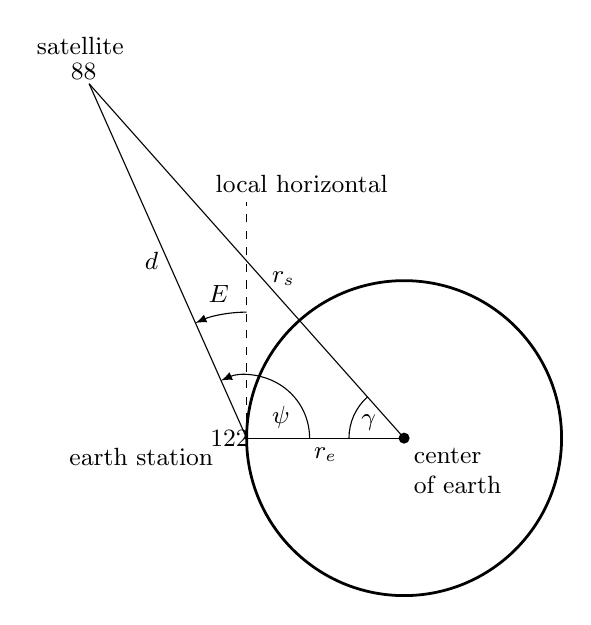
\begin{tikzpicture}[every node/.style={font=\small}]
   \draw [line width=1pt] (0,0) circle (2);
   \fill (0,0) circle (2pt);
   \node [below right,align=left] at (0,0) {center\\of earth};
   \draw (0,0) -- (-2,0) node[midway,below] {$r_e$};
   \node [below left] at (-2.3,0) {earth station};
   \draw (-2,0) -- (-4,4.5) node[midway,left] {$d$};
   \draw (0,0) -- (-4,4.5) node[pos=0.45,right] {$r_s$};
   \draw [dashed] (-2,0) -- (-2,3);
   \node [above] at (-1.3,3) {local horizontal};
   \draw [-latex] ([shift={(-2,0)}] 0:0.8) arc (0:113.96:0.8);
   \node [above right] at (-1.8,0) {$\psi$};
   \draw [-latex] ([shift={(-2,0)}] 90:1.6) arc (90:113.96:1.6);
   \node [above left] at (-2.1,1.6) {$E$};
   \node [left] at (-1.85,0) {\ding{122}};
   \node at ([shift={(-2,0)}] 113.96:5.1) {\ding{88}};
   \node [above] at ([shift={(-2,0)}] 113.96:5.2) {satellite};
   \draw (131.63:0.7) arc (131.63:180:0.7);
   \node at (-0.45,0.2) {$\gamma$};
  \end{tikzpicture}\vspace{-5mm}
 \end{center}
 \caption[]{}
 \label{fig:satellite}
\end{figure}

Use the Law of Cosines to show that
\begin{displaymath}
 d ~=~ r_s \,\sqrt{1 \;+\; \left( \frac{r_e}{r_s} \right)^2 \;-\; 2\,\left( \frac{r_e}{r_s} \right)
 \,\cos\;\gamma} ~~,
\end{displaymath}
and then use $E=\psi-90\Degrees$ and the Law of Sines to show that
\begin{displaymath}
 \cos\;E ~=~ \dfrac{\sin\;\gamma}{\sqrt{1 \;+\; \left( \dfrac{r_e}{r_s} \right)^2 \;-\;
  2\,\left( \dfrac{r_e}{r_s} \right) \,\cos\;\gamma}} ~.
\end{displaymath}
Note: This formula allows the angle of elevation $E$ to be calculated from the coordinates of the
earth station and the \emph{subsatellite point} (where the line from the satellite to the center of
the earth crosses the surface of the earth).\footnote{See pp. 22-25 in \textsc{T. Pratt and C.W.
Bostian}, \emph{Satellite Communications}, New York: John Wiley \& Sons, 1986.}
\end{enumerate}}
\newpage
%Begin Section 2.3
\section{The Law of Tangents}
We have shown how to solve a triangle in all four cases discussed at the beginning of this chapter.
An alternative to the Law of Cosines for Case 3 (two sides and the included angle) is the
\emph{Law of Tangents}:\index{Law of Tangents}

\statethm{thm:lawtangents}{
\textbf{Law of Tangents:} If a triangle has sides of lengths $a$, $b$, and $c$ opposite the angles
$A$, $B$, and $C$, respectively, then
\begin{align}
 \frac{a-b}{a+b} ~&=~
  \frac{\tan\;\frac{1}{2}(A-B)}{\tan\;\frac{1}{2}(A+B)}\label{eqn:lawtangentsab} ~,\\
 \frac{b-c}{b+c} ~&=~
  \frac{\tan\;\frac{1}{2}(B-C)}{\tan\;\frac{1}{2}(B+C)}\label{eqn:lawtangentsbc} ~,\\
 \frac{c-a}{c+a} ~&=~
  \frac{\tan\;\frac{1}{2}(C-A)}{\tan\;\frac{1}{2}(C+A)}\label{eqn:lawtangentsca} ~.
\end{align}}

Note that since $\tan\;(-\theta) = -\tan\;\theta$ for any angle $\theta$, we
can switch the order of the letters in each of the above formulas. For example, we can rewrite
formula (\ref{eqn:lawtangentsab}) as
\begin{equation}\label{eqn:lawtangentsba}
 \frac{b-a}{b+a}~=~\frac{\tan\;\frac{1}{2}(B-A)}{\tan\;\frac{1}{2}(B+A)}~,
\end{equation}
and similarly for the other formulas. If $a > b$, then it is usually more convenient to use
formula (\ref{eqn:lawtangentsab}), while formula (\ref{eqn:lawtangentsba}) is more convenient when
$b > a$.

\begin{exmp}\label{exmp:case3tangent}
\parpic[r]{\begin{tikzpicture}[scale=0.8,every node/.style={font=\small}]
 \fill [fillcolor] (0,0) -- (1.2,1.2) -- (3,0) -- cycle;
 \draw [linecolor,line width=1.5pt] (0,0) -- (1.2,1.2) node[black,midway,above left] {$b=3$} --
  (3,0) node[black,midway,above right] {$a=5$} -- cycle;
 \node [below] at (1.5,0) {$c$};
 \node [below left] at (0,0) {$A$};
 \node [below right] at (3,0) {$B$};
 \node [above] at (1.2,1.2) {$C=96\Degrees$};
\end{tikzpicture}}
\noindent \emph{Case 3: Two sides and the included angle.}\\Solve the triangle $\triangle\,ABC$ given
 $a =5$, $b = 3$, and $C = 96\Degrees$.\vspace{1mm}
 \par\noindent\textbf{Solution:} $A + B + C = 180\Degrees$, so $A + B = 180\Degrees - C =
 180\Degrees - 96\Degrees = 84\Degrees$. Thus, by the Law of Tangents,
 \begin{align*}
  \frac{a-b}{a+b} ~=~ \frac{\tan\;\frac{1}{2}(A-B)}{\tan\;\frac{1}{2}(A+B)} \quad&\Rightarrow\quad
   \frac{5-3}{5+3} ~=~ \frac{\tan\;\frac{1}{2}(A-B)}{\tan\;\frac{1}{2}(84\Degrees)}\\
  &\Rightarrow\quad \tan\;\tfrac{1}{2}(A-B) ~=~ \tfrac{2}{8}\tan\;42\Degrees ~=~ 0.2251\\
  &\Rightarrow\quad \tfrac{1}{2}(A-B) ~=~ 12.7\Degrees \quad\Rightarrow\quad A-B ~=~ 25.4\Degrees ~.
 \end{align*}
 We now have two equations involving $A$ and $B$, which we can solve by adding the equations:
 \begin{alignat*}{3}
  A &- B &&=\; 25.4\Degrees\\
  A &+ B &&=\; 84\Degrees\phantom{4\Degrees}\\[-2mm]
  --&--&&----\\[-2mm]
  2A &\phantom{+} &&=\; 109.4\Degrees \quad\Rightarrow\quad \boxed{A = 54.7\Degrees}
  \quad\Rightarrow\quad B ~=~ 84\Degrees - 54.7\Degrees \quad\Rightarrow\quad
  \boxed{B = 29.3\Degrees}
 \end{alignat*}
 We can find the remaining side $c$ by using the Law of Sines:
 \begin{displaymath}
  c ~=~ \frac{a\;\sin\;C}{\sin\;A} ~=~ \frac{5\;\sin\;96\Degrees}{\sin\;54.7\Degrees}
   \quad\Rightarrow\quad \boxed{c = 6.09}
 \end{displaymath}
\end{exmp}\vspace{-2mm}
\divider\vspace{-2mm}
\newpage
Note that in any triangle $\triangle\,ABC$, if $a = b$ then $A = B$ (why?), and so both sides of
formula (\ref{eqn:lawtangentsab}) would be $0$ (since $\tan\;0\Degrees = 0$). This means that
\emph{the Law of Tangents is of no help in Case 3 when the two known sides are equal}. For this
reason, and
perhaps also because of the somewhat unusual way in which it is used, the Law of Tangents seems to
have fallen out of favor in trigonometry books lately. It does not seem to have any advantages over
the Law of Cosines, which works even when the sides are equal, requires slightly fewer steps, and
is perhaps more straightforward.\footnote{Before the advent of electronic calculators, the Law of
Tangents was more popular than it is today
since it lent itself better than the Law of Cosines to what was known as
\emph{logarithmic computation}. In those days, computations with large numbers were handled by
taking logarithms and looking up values in a \emph{logarithm table}. Ratios (such as in the
Law of Tangents and the Law of Sines) could be replaced by differences of logarithms, making
computation easier.}

Related to the Law of Tangents are \emph{Mollweide's equations}:\footnote{Named after the German
astronomer and mathematician Karl Mollweide (1774-1825).}

\begin{center}\statecomment{\textbf{Mollweide's equations}: For any triangle $\triangle\,ABC$,
\begin{align}
 \frac{a-b}{c} ~&=~
  \frac{\sin\;\frac{1}{2}(A-B)}{\cos\;\frac{1}{2}C} ~,~\text{and}\label{eqn:mollweideamb}\\[4pt]
 \frac{a+b}{c} ~&=~
  \frac{\cos\;\frac{1}{2}(A-B)}{\sin\;\frac{1}{2}C} ~.\label{eqn:mollweideapb}
\end{align}}\end{center}

Note that all six parts of a triangle appear in both of Mollweide's equations. For this reason,
either equation can be used to check a solution of a triangle. If both sides of the equation agree
(more or less), then we know that the solution is correct.\index{Mollweide's equations}

\begin{exmp}
 Use one of Mollweide's equations to check the solution of the triangle from Example
 \ref{exmp:case3tangent}.\vspace{1mm}
 \par\noindent\textbf{Solution:} Recall that the full solution was $a=5$, $b=3$, $c=6.09$,
 $A=54.7\Degrees$, $B=29.3\Degrees$, and $C=96\Degrees$. We will check this with equation
 (\ref{eqn:mollweideamb}):
 \begin{align*}
 \frac{a-b}{c} ~&=~ \frac{\sin\;\frac{1}{2}(A-B)}{\cos\;\frac{1}{2}C}\\
 \frac{5-3}{6.09} ~&=~
  \frac{\sin\;\frac{1}{2}(54.7\Degrees - 29.3\Degrees)}{\cos\;\frac{1}{2}(96\Degrees)}\\
  \frac{2}{6.09} ~&=~ \frac{\sin\;12.7\Degrees}{\cos\;48\Degrees}\\
  0.3284 ~&=~ 0.3285 \quad\text{\ding{51}}
 \end{align*}
 The small difference ($\approx 0.0001$) is due to rounding errors from the
 original solution, so we can conclude that both sides of the equation agree, and hence the
 solution is correct.
\end{exmp}\vspace{-2mm}
\divider
\newpage
\begin{exmp}
 Can a triangle have the parts $a=6$, $b=7$, $c=9$, $A=55\Degrees$,
 $B=60\Degrees$, and $C=65\Degrees\;$?\vspace{1mm}
 \par\noindent\textbf{Solution:} Before using Mollweide's equations, simpler checks are that the
 angles add up to $180\Degrees$ and that the smallest and largest sides are opposite the smallest
 and largest angles, respectively. In this case all those conditions hold. So check with
 Mollweide's equation (\ref{eqn:mollweideapb}):
 \begin{align*}
 \frac{a+b}{c} ~&=~ \frac{\cos\;\frac{1}{2}(A-B)}{\sin\;\frac{1}{2}C}\\
 \frac{6+7}{9} ~&=~
  \frac{\cos\;\frac{1}{2}(55\Degrees - 60\Degrees)}{\sin\;\frac{1}{2}(65\Degrees)}\\
  \frac{13}{9} ~&=~ \frac{\cos\;(-2.5\Degrees)}{\sin\;32.5\Degrees}\\
  1.44 ~&=~ 1.86 \quad\text{\ding{55}}
 \end{align*}
 Here the difference is far too large, so we conclude that there is no triangle with these parts.
\end{exmp}\vspace{-2mm}
\divider
\vspace{1mm}

We will prove the Law of Tangents and Mollweide's equations in Chapter 3, where we will be able to
supply brief analytic proofs.\footnote{There are (complex) geometric proofs of the Law of
Tangents and Mollweide's equations. See pp. 96-98 in \textsc{P.R. Rider}, \emph{Plane and Spherical
Trigonometry}, New York: The Macmillan Company, 1942.}

\divider
\vspace{2mm}

\startexercises\label{sec2dot3}
\vspace{4mm}
{\small
\par\noindent For Exercises 1-3, use the Law of Tangents to solve the triangle $\triangle\,ABC$.
\begin{enumerate}[\bfseries 1.]
 \begin{multicols}{3}
  \item $a = 12$, $b = 8$, $C = 60\Degrees$
  \item $A = 30\Degrees$, $b = 4$, $c = 6$
  \item $a = 7$, $B = 60\Degrees$, $c = 9$
 \end{multicols}
\suspend{enumerate}
For Exercises 4-6, check if it is possible for a triangle to have the given parts.
\resume{enumerate}[{[\bfseries 1.]}]
 \item $a=5$, $b=7$, $c=10$, $A=27.7\Degrees$, $B=40.5\Degrees$, $C=111.8\Degrees$
 \item $a=3$, $b=7$, $c=9$, $A=19.2\Degrees$, $B=68.2\Degrees$, $C=92.6\Degrees$
 \item $a=6$, $b=9$, $c=9$, $A=39\Degrees$, $B=70.5\Degrees$, $C=70.5\Degrees$
 \item Let $\triangle\,ABC$ be a right triangle with $C=90\Degrees$. Show that
  $\;\tan\;\frac{1}{2}(A-B) =\frac{a-b}{a+b}\,$.
 \item For any triangle $\triangle\,ABC$, show that $\;\tan\;\frac{1}{2}(A-B) =
  \frac{a-b}{a+b}\;\cot\;\frac{1}{2}C\,$.
 \item For any triangle $\triangle\,ABC$, show that
  $\;\tan\;A = \dfrac{a\;\sin\;B}{c - a\;\cos\;B}\,$.
  (\emph{Hint: Draw the altitude from the vertex $C$ to $\overline{AB}$.}) Notice that this
  formula provides another way of solving a triangle in Case 3 (two sides and the included angle).
 \item For any triangle $\triangle\,ABC$, show that $\;c = b\;\cos\;A + a\;\cos\;B\,$. This is
  another check of a triangle.
 \item If $\,b\;\cos\;A = a\;\cos\;B\,$, show that the triangle $\triangle\,ABC$ is isosceles.
 \item Let $ABCD$ be a quadrilateral which completely contains its two diagonals. The quadrilateral
 has eight parts: four sides and four angles. What is the smallest number of parts that you would
 need to know to solve the quadrilateral? Explain your answer.
\end{enumerate}}
\newpage
%Begin Section 2.4
\section{The Area of a Triangle}
In elementary geometry you learned that the area of a triangle is one-half the base times the
height. We will now use that, combined with some trigonometry, to derive\index{area!triangle}
more formulas for the area when given various parts of the triangle.\vspace{2mm}

\par\noindent\emph{Case 1: Two sides and the included angle.}\\Suppose that we have a triangle
$\triangle\,ABC$, in which $A$ can be either acute, a right angle, or obtuse, as in Figure
\ref{fig:areacase1}. Assume that $A$, $b$, and $c$ are known.

\begin{figure}[h]
 \centering
 \subfloat[][ $A$ acute]{
  \begin{tikzpicture}[scale=1,every node/.style={font=\small}]
   \fill [fillcolor] (0,0) -- (1.8,1.2) -- (3,0) -- cycle;
   \draw [dashed] (1.8,1.2) -- (1.8,0) node[pos=0.4,left] {$h$};
   \draw (1.6,0) -- (1.6,0.2) -- (1.8,0.2);
   \draw [linecolor,line width=1.5pt] (0,0) -- (1.8,1.2) node[black,midway,above left] {$b$} --
    (3,0) node[black,midway,above right] {$a$} -- cycle;
   \node [below] at (0,0) {$A$};
   \node [above] at (1.8,1.2) {$C$};
   \node [below] at (3,0) {$B$};
   \node [below] at (1.5,0) {$c$};
  \end{tikzpicture}}
 \quad\quad
 \subfloat[][ $A = 90\Degrees$]{
  \begin{tikzpicture}[scale=1,every node/.style={font=\small}]
   \fill [fillcolor] (0,0) -- (0,1.2) -- (3,0) -- cycle;
   \draw (0.2,0) -- (0.2,0.2) -- (0,0.2);
   \draw [linecolor,line width=1.5pt] (0,0) -- (0,1.2) node[black,midway,left] {$b$}
    node[black,midway,right] {$h$} -- (3,0) node[black,midway,above right] {$a$} -- cycle;
   \node [below] at (0,0) {$A$};
   \node [above] at (0,1.2) {$C$};
   \node [below] at (3,0) {$B$};
   \node [below] at (1.5,0) {$c$};
  \end{tikzpicture}}
 \quad\quad
 \subfloat[][ $A$ obtuse]{
  \begin{tikzpicture}[scale=1,every node/.style={font=\small}]
   \fill [fillcolor] (0,0) -- (-1,1.2) -- (2.5,0) -- cycle;
   \draw [dashed] (-1.07,1.2) -- (-1.07,0) node[midway,left] {$h$} -- (0,0);
   \draw (-0.87,0) -- (-0.87,0.2) -- (-1.07,0.2);
   \draw [linecolor,line width=1.5pt] (0,0) -- (-1,1.2) node[black,pos=0.35,left] {$b$} --
    (2.5,0) node[black,midway,above right] {$a$} -- cycle;
   \node [below] at (0,0) {$A$};
   \node [above] at (-1,1.2) {$C$};
   \node [below] at (2.5,0) {$B$};
   \node [below] at (1.25,0) {$c$};
  \end{tikzpicture}}\vspace{-2mm}
 \caption[]{\quad Area of $\triangle\,ABC$}
 \label{fig:areacase1}
\end{figure}

In each case we draw an altitude of height $h$ from the vertex at $C$ to $\overline{AB}$, so that
the area (which we will denote by the letter $K$) is given by $K = \frac{1}{2}hc$. But we see that
$h = b\;\sin\;A$ in each of the triangles (since $\;h=b$ and $\sin\;A =
\sin\;90\Degrees = 1$ in Figure \ref{fig:areacase1}(b), and $\;h = b\;\sin\;(180\Degrees - A) =
b\;\sin\;A$ in Figure \ref{fig:areacase1}(c)). We thus get the following formula:
\begin{empheq}[box=\widefbox]{equation}
 \text{Area} ~=~ K ~=~ \tfrac{1}{2}\,bc\;\sin\;A\label{eqn:areacase1a}
\end{empheq}
The above formula for the area of $\triangle\,ABC$ is in terms of the known parts
$A$, $b$, and $c$. Similar arguments for the angles $B$ and $C$ give us:
\begin{empheq}[box=\widefbox]{alignat=3}
 \text{Area} ~&=~ K ~&&=~ \tfrac{1}{2}\,ac\;\sin\;B\label{eqn:areacase1b}\\
 \text{Area} ~&=~ K ~&&=~ \tfrac{1}{2}\,ab\;\sin\;C\label{eqn:areacase1c}
\end{empheq}
Notice that the height $h$ does not appear explicitly in these formulas, although it is implicitly
there. These formulas have the advantage of being in terms of parts of the triangle, without having
to find $h$ separately.\index{triangle!area}

\begin{exmp}\label{exmp:areacase1}
\parpic[r]{\begin{tikzpicture}[scale=0.8,every node/.style={font=\small}]
 \fill [fillcolor] (0,0) -- (1.8,1.2) -- (3,0) -- cycle;
 \draw [linecolor,line width=1.5pt] (0,0) -- (1.8,1.2) node[black,midway,above left] {$b=5$} --
  (3,0) node[black,midway,above right] {$a$} -- cycle;
 \node [below] at (1.5,0) {$c=7$};
 \node [below left] at (0,0) {$A=33\Degrees$};
 \node [below right] at (3,0) {$B$};
 \node [above] at (1.8,1.2) {$C$};
\end{tikzpicture}}
\noindent Find the area of the triangle $\triangle\,ABC$ given\\$A = 33\Degrees$, $b = 5$, and
 $c = 7$.\vspace{1mm}
 \par\noindent\textbf{Solution:} Using formula (\ref{eqn:areacase1a}), the area $K$ is given by:
 \begin{align*}
  K ~&=~ \tfrac{1}{2}\,bc\;\sin\;A\\
   &=~ \tfrac{1}{2}\,(5)(7)\;\sin\;33\Degrees\\
  K ~&=~ 9.53
 \end{align*}
\end{exmp}\vspace{-2mm}
\divider
\newpage
\noindent\emph{Case 2: Three angles and any side.}\\Suppose that we have a triangle
$\triangle\,ABC$ in which one side, say, $a$, and all three angles are known.\footnote{Note that
this is equivalent to knowing just \emph{two} angles and a side (why?).} By the Law of Sines we
know that
\begin{displaymath}
 c ~=~ \frac{a\;\sin\;C}{\sin\;A} ~,
\end{displaymath}
so substituting this into formula (\ref{eqn:areacase1b}) we get:
\begin{empheq}[box=\widefbox]{equation}
 \text{Area} ~=~ K ~=~ \frac{a^2 \;\sin\;B \;\sin\;C}{2\;\sin\;A}\label{eqn:areacase2a}
\end{empheq}
Similar arguments for the sides $b$ and $c$ give us:
\begin{empheq}[box=\widefbox]{alignat=3}
 \text{Area} ~&=~ K ~&&=~ \frac{b^2 \;\sin\;A \;\sin\;C}{2\;\sin\;B}\label{eqn:areacase2b}\\
 \text{Area} ~&=~ K ~&&=~ \frac{c^2 \;\sin\;A \;\sin\;B}{2\;\sin\;C}\label{eqn:areacase2c}
\end{empheq}

\begin{exmp}\label{exmp:areacase2}
\parpic[r]{\begin{tikzpicture}[scale=0.8,every node/.style={font=\small}]
 \fill [fillcolor] (0,0) -- (-1,1.2) -- (2.5,0) -- cycle;
 \draw [linecolor,line width=1.5pt] (0,0) -- (-1,1.2) node[black,pos=0.35,left] {$b$} --
  (2.5,0) node[black,midway,above right] {$a=12$} -- cycle;
 \node [below] at (0,0) {$A=115\Degrees$};
 \node [above] at (-1,1.2) {$C=40\Degrees$};
 \node [below] at (2.5,0) {$B=25\Degrees$};
 \node [below] at (1.25,0) {$c$};
 \end{tikzpicture}}
\noindent Find the area of the triangle $\triangle\,ABC$ given\\$A = 115\Degrees$, $B=25\Degrees$,
 $C=40\Degrees$, and $a = 12$.\vspace{1mm}
 \par\noindent\textbf{Solution:} Using formula (\ref{eqn:areacase2a}), the area $K$ is given by:
 \begin{align*}
  K ~&=~ \frac{a^2 \;\sin\;B \;\sin\;C}{2\;\sin\;A}\\
   &=~ \frac{12^2 \;\sin\;25\Degrees \;\sin\;40\Degrees}{2\;\sin\;115\Degrees}\\
  K ~&=~ 21.58
 \end{align*}
\end{exmp}\vspace{-2mm}
\divider
\vspace{2mm}

\noindent\emph{Case 3: Three sides.}\\Suppose that we have a triangle $\triangle\,ABC$ in which all
three sides are known. Then \emph{Heron's formula}\footnote{Due to the ancient Greek engineer and
mathematician Heron of Alexandria (c. 10-70 A.D.).}\index{Heron's formula} gives us the area:

\begin{center}\statecomment{\textbf{Heron's formula:} For a triangle $\triangle\,ABC$ with sides
$a$, $b$, and $c$, let $s = \frac{1}{2}\,(a+b+c)$ (i.e. $2s = a+b+c$ is the perimeter of the
triangle). Then the area $K$ of the triangle is
\begin{equation}\label{eqn:heron}
 \text{Area} ~=~ K ~=~ \sqrt{s\,(s-a)\,(s-b)\,(s-c)} ~~.
\end{equation}}\end{center}

To prove this, first remember that the area $K$ is one-half the base times the height. Using $c$ as
the base and the altitude $h$ as the height, as before in Figure \ref{fig:areacase1}, we have
$K = \frac{1}{2}hc$. Squaring both sides gives us
\begin{equation}\label{eqn:heronproof1}
 K^2 = \tfrac{1}{4}\,h^2 c^2 ~.
\end{equation}
\newpage
In Figure \ref{fig:heron}, let $D$ be the point where the altitude touches $\overline{AB}$ (or its
extension).

\begin{figure}[h]
 \centering
 \subfloat[][ $A$ acute]{
  \begin{tikzpicture}[scale=1,every node/.style={font=\small}]
   \fill [fillcolor] (0,0) -- (1.8,1.2) -- (3,0) -- cycle;
   \draw [dashed] (1.8,1.2) -- (1.8,0) node[pos=0.4,left] {$h$};
   \draw (1.6,0) -- (1.6,0.2) -- (1.8,0.2);
   \draw [linecolor,line width=1.5pt] (0,0) -- (1.8,1.2) node[black,midway,above left] {$b$} --
    (3,0) node[black,midway,above right] {$a$} -- cycle;
   \node [below] at (0,0) {$A$};
   \node [above] at (1.8,1.2) {$C$};
   \node [below] at (3,0) {$B$};
   \node [below] at (1.3,0) {$c$};
   \node [below] at (1.8,0) {$D$};
  \end{tikzpicture}}
 \qquad\qquad
 \subfloat[][ $A$ obtuse]{
  \begin{tikzpicture}[scale=1,every node/.style={font=\small}]
   \fill [fillcolor] (0,0) -- (-1,1.2) -- (2.5,0) -- cycle;
   \draw [dashed] (-1.07,1.2) -- (-1.07,0) node[midway,left] {$h$} -- (0,0);
   \draw (-0.87,0) -- (-0.87,0.2) -- (-1.07,0.2);
   \draw [linecolor,line width=1.5pt] (0,0) -- (-1,1.2) node[black,pos=0.35,left] {$b$} --
    (2.5,0) node[black,midway,above right] {$a$} -- cycle;
   \node [below] at (0,0) {$A$};
   \node [above] at (-1,1.2) {$C$};
   \node [below] at (2.5,0) {$B$};
   \node [below] at (1.25,0) {$c$};
   \node [below] at (-1.07,0) {$D$};
  \end{tikzpicture}}\vspace{-2mm}
 \caption[]{\quad Proof of Heron's formula}
 \label{fig:heron}
\end{figure}

\noindent By the Pythagorean Theorem, we see that $\;h^2 = b^2 - (AD)^2$. In Figure
\ref{fig:heron}(a), we see that $\;AD = b\;\cos\;A$. And in Figure \ref{fig:heron}(b) we see that
$\;AD = b\;\cos\;(180\Degrees - A) = -b\cos\;A$. Hence, in either case we have
$\;(AD)^2 = b^2 \;(\cos\;A)^2$, and so
\begin{equation}\label{eqn:heronproof2}
 h^2 ~=~ b^2 - b^2 \;(\cos\;A)^2 ~=~ b^2 \,(1 - (\cos\;A)^2 ) ~=~ b^2 \,(1+ \cos\;A)\,(1- \cos\;A)~.
\end{equation}
(Note that the above equation also holds when $A=90\Degrees$ since $\cos\;90\Degrees =0$ and $h=b$).
Thus, substituting equation (\ref{eqn:heronproof2}) into equation (\ref{eqn:heronproof1}), we have
\begin{equation}\label{eqn:heronproof3}
 K^2 = \tfrac{1}{4}\,b^2 c^2 \,(1+ \cos\;A)\,(1- \cos\;A) ~.
\end{equation}
By the Law of Cosines we know that
\begin{align*}
 1 + \cos\;A ~&=~ 1 + \frac{b^2 + c^2 - a^2}{2bc} ~=~ \frac{2bc + b^2 + c^2 - a^2}{2bc}
  ~=~ \frac{(b+c)^2 - a^2}{2bc} ~=~ \frac{((b+c) + a)\,((b+c) - a)}{2bc}\\
  &=~ \frac{(a + b + c)\,(b + c - a)}{2bc} ~,
\end{align*}
and similarly
\begin{align*}
 1 - \cos\;A ~&=~ 1 - \frac{b^2 + c^2 - a^2}{2bc} ~=~ \frac{2bc - b^2 - c^2 + a^2}{2bc}
  ~=~ \frac{a^2 - (b-c)^2}{2bc} ~=~ \frac{(a - (b-c))\,(a + (b-c))}{2bc}\\
  &=~ \frac{(a - b + c)\,(a + b - c)}{2bc} ~.
\end{align*}
Thus, substituting these expressions into equation (\ref{eqn:heronproof3}), we have
\begin{align*}
 K^2 ~&=~ \tfrac{1}{4}\,b^2 c^2 \;\frac{(a + b + c)\,(b + c - a)}{2bc} \;\cdot\;
  \frac{(a - b + c)\,(a + b - c)}{2bc}\\
  &=~ \frac{a + b + c}{2} \;\cdot\; \frac{b + c - a}{2} \;\cdot\; \frac{a - b + c}{2} \;\cdot\;
   \frac{a + b - c}{2} ~,\\
 \intertext{and since we defined $s = \frac{1}{2}\,(a+b+c)$, we see that}
  K^2 ~&=~ s\,(s-a)\,(s-b)\,(s-c) ~,\\
 \intertext{so upon taking square roots we get}
 K ~&=~ \sqrt{s\,(s-a)\,(s-b)\,(s-c)} ~~.\quad\qed
\end{align*}
\newpage
\begin{exmp}\label{exmp:heron}
\parpic[r]{\begin{tikzpicture}[scale=0.8,every node/.style={font=\small}]
 \fill [fillcolor] (0,0) -- (1.2,1.2) -- (3,0) -- cycle;
 \draw [linecolor,line width=1.5pt] (0,0) -- (1.2,1.2) node[black,midway,above left] {$b=4$} --
  (3,0) node[black,midway,above right] {$a=5$} -- cycle;
 \node [below] at (1.5,0) {$c=7$};
 \node [below left] at (0,0) {$A$};
 \node [below right] at (3,0) {$B$};
 \node [above] at (1.2,1.2) {$C$};
\end{tikzpicture}}
\noindent Find the area of the triangle $\triangle\,ABC$ given $a=5$, $b=4$, and $c = 7$.\vspace{1mm}
 \par\noindent\textbf{Solution:} Using Heron's formula with $s = \frac{1}{2}\,(a+b+c) =
 \frac{1}{2}\,(5+4+7) = 8$, the area $K$ is given by:
 \begin{align*}
  K ~&=~ \sqrt{s\,(s-a)\,(s-b)\,(s-c)}\\
   &=~ \sqrt{8\,(8-5)\,(8-4)\,(8-7)} ~=~ \sqrt{96} \quad\Rightarrow\quad \boxed{K ~=~ 4\,\sqrt{6}
   ~\approx~ 9.8} ~.
 \end{align*}
\end{exmp}\vspace{-3mm}
\divider
\vspace{1mm}

Heron's formula is useful for theoretical purposes (e.g. in deriving other formulas).
However, it is not well-suited for calculator use, exhibiting what is
called \emph{numerical instability}\index{numerical instability}\index{Heron's formula!numerical
instability of} for ``extreme'' triangles, as in the following example.

\begin{exmp}\label{exmp:heronfail}
 Find the area of the triangle $\triangle\,ABC$ given $a=1000000$, $b=999999.9999979$, and
 $c = 0.0000029$.\vspace{1mm}
 \par\noindent\textbf{Solution:} To use Heron's formula, we need to calculate
 $s = \frac{1}{2}\,(a+b+c)$. Notice that the actual value of $a+b+c$ is $2000000.0000008$, which
 has $14$ digits. Most calculators can store $12$-$14$ digits internally (even if they display
 less), and hence may round off that value of $a+b+c$ to $2000000$. When we then divide that
 rounded value for $a+b+c$ by $2$ to get $s$, some calculators (e.g. the TI-83 Plus) will give a
 rounded down value of $1000000$.
 
 This is a problem because $a=1000000$, and so we would get $s-a=0$, causing Heron's formula to
 give us an area of $0$ for the triangle! And this is indeed the incorrect answer that the TI-83
 Plus returns. Other calculators may give some other inaccurate
 answer, depending on how they store values internally. The actual area - accurate to $15$
 decimal places - is $K = 0.99999999999895$, i.e. it is basically $1$.
\end{exmp}\vspace{-3mm}
\divider
\vspace{1mm}

The above example shows how problematic \emph{floating-point arithmetic} can be.\footnote{This is
an issue even on modern computers. There is an
excellent overview of this important subject in the article \emph{What Every Computer
Scientist Should Know About Floating-Point Arithmetic} by D. Goldberg, available at
\url{http://docs.sun.com/source/806-3568/ncg_goldberg.html}} Luckily there is a better
formula\footnote{Due to W. Kahan: \url{http://www.eecs.berkeley.edu/~wkahan/Triangle.pdf}} for
the area of a triangle when the three sides are known:

\begin{center}\statecomment{For a triangle $\triangle\,ABC$ with sides $a \ge b \ge c$, the area is:
\begin{equation}\label{eqn:kahan}
  \text{Area} ~=~ K ~=~ \tfrac{1}{4}\,\sqrt{(a + (b+c))\,(c - (a-b))\,(c + (a-b))\,(a + (b-c))}
\end{equation}}\end{center}

To use this formula, sort the names of the sides so that
$a \ge b \ge c$. Then perform the operations inside the square root \emph{in the exact order in
which they appear in the formula, including the use of parentheses}. Then take the square root and
divide by $4$. For the triangle in Example \ref{exmp:heronfail}, the above formula gives an
answer of exactly $K = 1$ on the same TI-83 Plus calculator that failed with Heron's
formula.
What is amazing about this formula is that it is just Heron's formula rewritten! The use of
parentheses is what forces the correct order of operations for numerical stability.
\newpage
Another formula\footnote{Due to the Chinese mathematician Qiu Jiushao (ca. 1202-1261).} for the
area of a triangle given its three sides is given below:

\begin{center}\statecomment{For a triangle $\triangle\,ABC$ with sides $a \ge b \ge c$, the area is:
\begin{equation}\label{eqn:jiushao}
  \text{Area} ~=~ K ~=~ \tfrac{1}{2}\,\sqrt{a^2 c^2 ~-~ \left( \tfrac{a^2 + c^2 - b^2}{2} \right)^2}
\end{equation}}\end{center}

For the triangle in Example \ref{exmp:heronfail}, the above formula gives an answer of
exactly $K = 1$ on the same TI-83 Plus calculator that failed with Heron's formula.

\divider
\vspace{2mm}

\startexercises\label{sec2dot4}
\vspace{5mm}
{\small
\par\noindent For Exercises 1-6, find the area of the triangle $\triangle\,ABC$.
\begin{enumerate}[\bfseries 1.]
 \begin{multicols}{2}
  \item $A = 70\Degrees$, $b = 4$, $c = 12$
  \item $a = 10$, $B = 95\Degrees$, $c = 35$
 \end{multicols}
 \begin{multicols}{2}
  \item $A = 10\Degrees$, $B = 48\Degrees$, $C = 122\Degrees$, $c = 11$
  \item $A = 171\Degrees$, $B = 1\Degrees$, $C = 8\Degrees$, $b = 2$
 \end{multicols}
 \begin{multicols}{2}
  \item $a = 2$, $b = 3$, $c = 4$
  \item $a = 5$, $b=6$, $c = 5$
 \end{multicols}
 \item\label{exer:areaquad} Find the area of the quadrilateral in Figure \ref{fig:areaquad}
  below.\vspace{-2mm}
\begin{figure}[h]
\begin{minipage}[t]{7.5cm}
 \begin{center}
  \begin{tikzpicture}[scale=1.2,every node/.style={font=\small}]
   \filldraw [linecolor,fill=fillcolor,line width=1.5pt] (0,0) -- (-0.5,1)
    node[black,pos=0.7,below left] {$2$} -- (2,2) node[black,midway,above] {$4$} -- (4,1)
    node[black,pos=0.4,above right] {$3.5$} -- cycle;
   \draw [dashed,latex-latex] (-0.47,1) -- (3.93,1) node[pos=0.5,fill=fillcolor] {$6$};
   \node [below] at (2,0.5) {$5.5$};
  \end{tikzpicture}\vspace{-5mm}
 \end{center}
 \caption[]{\quad Exercise \ref{exer:areaquad}}
 \label{fig:areaquad}
\end{minipage}
\begin{minipage}[t]{7.5cm}
 \begin{center}
  \begin{tikzpicture}[every node/.style={font=\small}]
   \fill [fillcolor] (0,0) -- (-0.5,1) -- (2,2) -- (4,1) -- cycle;
   \draw [name path=d1] (0,0) -- (2,2);
   \draw [name path=d2] (-0.5,1) -- (4,1);
   \draw [linecolor,line width=1.5pt] node[black,left] {$A$} (0,0) -- (-0.5,1) 
    node[black,left] {$B$} -- (2,2) node[black,above] {$C$} -- (4,1) node[black,right] {$D$}
	-- cycle;
   \draw [name intersections={of=d1 and d2}] ([shift={(intersection-1)}] 0:0.4) arc (0:45:0.4);
   \node [above] at (1.6,1) {$\theta$};
  \end{tikzpicture}\vspace{-5mm}
 \end{center}
 \caption[]{\quad Exercise \ref{exer:areaquaddiag}}
 \label{fig:areaquaddiag}
\end{minipage}
\end{figure}\vspace{-2mm}
 \item\label{exer:areaquaddiag} Let $ABCD$ be a quadrilateral which completely contains its two
  diagonals,
  as in Figure \ref{fig:areaquaddiag} above. Show that the area $K$ of $ABCD$ is equal to half the
  product of its diagonals and the sine of the angle they form, i.e. $K =
  \frac{1}{2}\,AC\,\cdot\,BD\;\sin\;\theta\;$.
 \item From formula (\ref{eqn:areacase2a}) derive the following formula for the area of a triangle
  $\triangle\,ABC$:
  \begin{displaymath}
   \text{Area} ~=~ K ~=~ \frac{a^2 \;\sin\;B \;\sin\;C}{2\;\sin\;(B+C)}
  \end{displaymath}
 \item Show that the triangle area formula
  \begin{displaymath}
   \text{Area} ~=~ K ~=~ \tfrac{1}{4}\,\sqrt{(a + (b+c))\,(c - (a-b))\,(c + (a-b))\,(a + (b-c))}
  \end{displaymath}
  is equivalent to Heron's formula. (\emph{Hint: In Heron's formula replace $s$ by
  $\frac{1}{2}(a+b+c)$.})
 \item\label{exmp:jiushao} Show that the triangle area formula (\ref{eqn:jiushao})
  is equivalent to Heron's formula. (\emph{Hint: Factor the expression inside the square root.})
 \item Find the angle $A$ in Example \ref{exmp:heronfail}, then use formula (\ref{eqn:areacase1a})
  to find the area. Did it work?
\end{enumerate}}
\newpage
%Begin Section 2.5
\section{Circumscribed and Inscribed Circles}
Recall from the Law of Sines that any triangle $\triangle\,ABC$ has a common ratio of sides to
sines of opposite angles, namely
\begin{displaymath}
 \frac{a}{\sin\;A} ~=~ \frac{b}{\sin\;B} ~=~ \frac{c}{\sin\;C} ~.
\end{displaymath}
This common ratio has a geometric meaning: it is the
diameter (i.e. twice the radius) of the unique circle in which $\triangle\,ABC$ can be
inscribed,\index{inscribed triangle} called the\index{triangle!inscribed}
\textbf{circumscribed circle}\index{circumscribed circle}\index{circle!circumscribed} of the
triangle. Before proving this, we need to review some elementary geometry.

A \textbf{central angle}\index{central angle}\index{angle!central} of a circle is an angle whose
vertex is the center $O$ of the circle and whose sides (called \textbf{radii})\index{radius}
are line segments from $O$ to two points on the circle.
In Figure \ref{fig:angletypes}(a), $\angle\,O$ is a central angle and we say that it
\emph{intercepts the arc} $\wideparen{BC}$.\index{arc}

\begin{figure}[h]
 \centering
 \subfloat[][ Central angle $\angle\,O$]{
  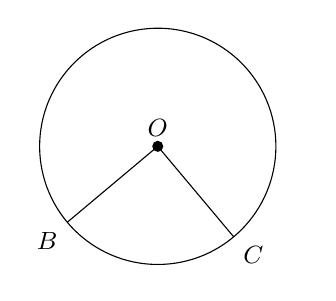
\begin{tikzpicture}[scale=1,every node/.style={font=\small}]
   \draw (0,0) circle (1.5);
   \fill (0,0) circle (2pt);
   \node [above] at (0,0) {$O$};
   \draw (0,0) -- (-140:1.5);
   \node [below left] at (-140:1.5) {$B$};
   \draw (0,0) -- (-50:1.5);
   \node [below right] at (-50:1.5) {$C$};
   \draw [white] (1.5,1.5) -- (1.9,1.5);
  \end{tikzpicture}}
 \qquad\qquad
 \subfloat[][ Inscribed angle $\angle\,A$]{
  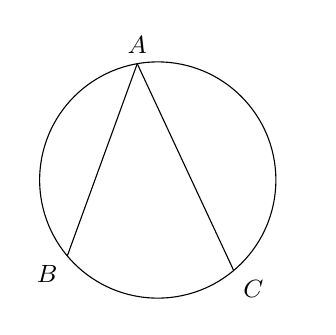
\begin{tikzpicture}[scale=1,every node/.style={font=\small}]
   \draw (0,0) circle (1.5);
   \node [above] at (100:1.5) {$A$};
   \draw (100:1.5) -- (-140:1.5);
   \node [below left] at (-140:1.5) {$B$};
   \draw (100:1.5) -- (-50:1.5);
   \node [below right] at (-50:1.5) {$C$};
   \draw [white] (1.5,1.5) -- (1.9,1.5);
  \end{tikzpicture}}
 \qquad\qquad
 \subfloat[][ $\angle\,A = \angle\,D = \frac{1}{2}\,\angle\,O$]{
  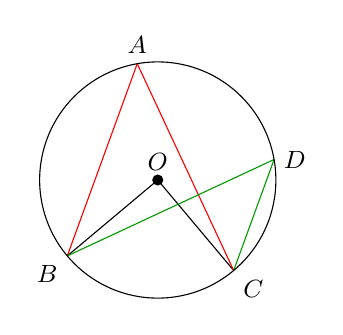
\begin{tikzpicture}[scale=1,every node/.style={font=\small}]
   \fill (0,0) circle (2pt);
   \node [above] at (0,0) {$O$};
   \draw (0,0) -- (-140:1.5);
   \node [below left] at (-140:1.5) {$B$};
   \draw (0,0) -- (-50:1.5);
   \node [below right] at (-50:1.5) {$C$};
   \node [above] at (100:1.5) {$A$};
   \draw [red] (100:1.5) -- (-140:1.5);
   \draw [red] (100:1.5) -- (-50:1.5);
   \node [right] at (10:1.5) {$D$};
   \draw [green!60!black] (10:1.5) -- (-140:1.5);
   \draw [green!60!black] (10:1.5) -- (-50:1.5);
   \draw (0,0) circle (1.5);
  \end{tikzpicture}}\vspace{-2mm}
 \caption[]{\quad Types of angles in a circle}
 \label{fig:angletypes}
\end{figure}

An \textbf{inscribed angle}\index{inscribed angle}\index{angle!inscribed} of a circle is an angle
whose vertex is a point $A$ on the circle and whose sides are line segments (called \textbf{chords})
from $A$ to two other points on the circle. In Figure \ref{fig:angletypes}(b),\index{chord}
$\angle\,A$ is an inscribed angle that intercepts the arc $\wideparen{BC}$. We state here without
proof\footnote{For a proof, see pp. 210-211 in \textsc{R.A. Avery}, \emph{Plane Geometry}, Boston:
Allyn \& Bacon, 1950.} a useful relation between inscribed and central angles:

\statethm{thm:centralangle}{If an inscribed angle $\angle\,A$ and a central angle $\angle\,O$
intercept the same arc, then $\angle\,A = \frac{1}{2}\,\angle\,O\,$. Thus, inscribed
angles which intercept the same arc are equal.}

Figure \ref{fig:angletypes}(c) shows two inscribed angles, $\angle\,A$ and $\angle\,D$, which
intercept the same arc $\wideparen{BC}$ as the central angle $\angle\,O$, and hence
$\angle\,A = \angle\,D = \frac{1}{2}\,\angle\,O$ (so $\;\angle\,O = 2\,\angle\,A =
2\,\angle\,D\,)$.

We will now prove our assertion about the common ratio in the Law of Sines:

\statethm{thm:circumscribedradius}{For any triangle $\triangle\,ABC$, the radius $R$ of its
circumscribed circle is given by:
\begin{equation}\label{eqn:circumscribedradius}
 2\,R ~=~ \frac{a}{\sin\;A} ~=~ \frac{b}{\sin\;B} ~=~ \frac{c}{\sin\;C}
\end{equation}}

\noindent (Note: For a circle of diameter $1$, this means $a=\sin\;A$, $b=\sin\;B$, and
$c=\sin\;C$.)
\newpage
To prove this, let $O$ be the center of the circumscribed circle for a triangle $\triangle\,ABC$.
Then $O$ can be either inside, outside, or on the triangle, as in Figure
\ref{fig:circumscribedradius} below. In the first two cases, draw a perpendicular line segment
from $O$ to $\overline{AB}$ at the point $D$.

\begin{figure}[h]
 \centering
 \subfloat[][ $O$ inside $\triangle\,ABC$]{
  \begin{tikzpicture}[scale=1,every node/.style={font=\small}]
   \fill [fillcolor] (-40:2) -- (100:2) -- (220:2) -- (-40:2);
   \draw [dashed] (0,-1.285) -- (0,0);
   \node [below] at (0,-1.285) {$D$};
   \draw (0.2,-1.285) -- (0.2,-1.085) -- (0,-1.085);
   \fill (0,0) circle (2pt);
   \node [above] at (0,0) {$O$};
   \draw [linecolor,line width=1.5pt] (100:2) -- (220:2) node[black,midway,left] {$b$};
   \node [above] at (100:2) {$C$};
   \draw [linecolor,line width=1.5pt] (100:2) -- (-40:2) node[black,midway,right] {$a$};
   \node [below right] at (-40:2) {$B$};
   \node [below left] at (220:2) {$A$};
   \draw [linecolor,line width=1.5pt] (220:2) -- (-40:2) node[black,pos=0.3,below] {$\frac{c}{2}$}
    node[black,pos=0.7,below] {$\frac{c}{2}$};
   \draw [dashed] (0,0) -- (220:2) node[midway,above] {$R$};
   \draw [dashed] (0,0) -- (-40:2) node[midway,above] {$R$};
   \draw [line width=1pt] (0,0) circle (2);
  \end{tikzpicture}}
 \enskip
 \subfloat[][ $O$ outside $\triangle\,ABC$]{
  \begin{tikzpicture}[scale=1,every node/.style={font=\small}]
   \fill [fillcolor] (20:2) -- (100:2) -- (160:2) -- (20:2);
   \draw [dashed] (0,0.684) -- (0,0);
   \node [above] at (0,0.684) {$D$};
   \draw (0.2,0.684) -- (0.2,0.484) -- (0,0.484);
   \fill (0,0) circle (2pt);
   \node [below] at (0,0) {$O$};
   \draw [linecolor,line width=1.5pt] (100:2) -- (160:2) node[black,pos=0.4,right] {$b$};
   \node [above] at (100:2) {$C$};
   \draw [linecolor,line width=1.5pt] (100:2) -- (20:2) node[black,midway,above] {$a$};
   \node [right] at (20:2) {$B$};
   \node [left] at (160:2) {$A$};
   \draw [linecolor,line width=1.5pt] (160:2) -- (20:2) node[black,pos=0.35,above] {$\frac{c}{2}$}
    node[black,pos=0.65,above] {$\frac{c}{2}$};
   \draw [dashed] (0,0) -- (160:2) node[midway,below] {$R$};
   \draw [dashed] (0,0) -- (20:2) node[midway,below] {$R$};
   \draw [line width=1pt] (0,0) circle (2);
  \end{tikzpicture}}
 \enskip
 \subfloat[][ $O$ on $\triangle\,ABC$]{
  \begin{tikzpicture}[scale=1,every node/.style={font=\small}]
   \fill [fillcolor] (0:2) -- (100:2) -- (180:2) -- (0:2);
   \node [below] at (0,0) {$O$};
   \draw [linecolor,line width=1.5pt] (100:2) -- (180:2) node[black,pos=0.4,left] {$b$};
   \node [above] at (100:2) {$C$};
   \draw [linecolor,line width=1.5pt] (100:2) -- (0:2) node[black,midway,above] {$a$};
   \node [right] at (0:2) {$B$};
   \node [left] at (180:2) {$A$};
   \draw [linecolor,line width=1.5pt] (180:2) -- (0:2) node[black,pos=0.45,above] {$c$};
   \node [below] at (-1,0) {$R$};
   \node [below] at (1,0) {$R$};
   \draw [line width=1pt] (0,0) circle (2);
   \fill (0,0) circle (2pt);
  \end{tikzpicture}}\vspace{-2mm}
 \caption[]{\quad Circumscribed circle for $\triangle\,ABC$}
 \label{fig:circumscribedradius}
\end{figure}

The radii $\overline{OA}$ and $\overline{OB}$ have the same length $R$, so $\triangle\,AOB$ is an
isosceles triangle. Thus, from elementary geometry we know that $\overline{OD}$ bisects both the
angle $\angle\,AOB$ and the side $\overline{AB}$. So $\angle\,AOD = \frac{1}{2}\,\angle\,AOB$
and $AD = \frac{c}{2}$. But since the inscribed angle $\angle\,ACB$ and the central angle
$\angle\,AOB$ intercept the same arc $\wideparen{AB}$, we know from Theorem \ref{thm:centralangle}
that $\angle\,ACB = \frac{1}{2}\,\angle\,AOB$. Hence, $\angle\,ACB = \angle\,AOD$. So since $C =
\angle\,ACB$, we have
\begin{displaymath}
 \sin\;C ~=~ \sin\;\angle\,AOD ~=~ \frac{AD}{OA} ~=~ \frac{\frac{c}{2}}{R} ~=~ \frac{c}{2R}
 \quad\Rightarrow\quad 2\,R ~=~ \frac{c}{\sin\;C} ~,
\end{displaymath}
so by the Law of Sines the result follows if $O$ is inside or outside $\triangle\,ABC$.

Now suppose that $O$ is on $\triangle\,ABC$, say, on the side $\overline{AB}$, as in
Figure \ref{fig:circumscribedradius}(c). Then $\overline{AB}$ is a diameter of the circle, so
$C = 90\Degrees$ by Thales' Theorem. Hence, $\sin\;C = 1$, and so
$2\,R = AB = c = \frac{c}{1} = \frac{c}{\sin\;C}\;$,
and the result again follows by the Law of Sines. $\qed$\vspace{-1mm}

\begin{exmp}
\piccaption[]{\label{fig:circum345}}\parpic[r]{\begin{tikzpicture}[every node/.style={font=\small}]
 \fill [fillcolor] (0,0) -- (2,0) -- (2,1.5) -- (0,0);
 \draw (1.8,0) -- (1.8,0.2) -- (2,0.2);
 \draw [linecolor,line width=1.5pt] (0,0) -- (2,0) node[black,midway,below] {$4$};
 \draw [linecolor,line width=1.5pt] (0,0) -- (2,1.5) node[black,pos=0.5,above] {$5$};
 \draw [linecolor,line width=1.5pt] (2,0) -- (2,1.5) node[black,pos=0.4,left] {$3$};
 \draw [line width=1pt] (1,0.75) circle (1.25);
 \fill (1,0.75) circle (2pt);
 \node [below] at (1,0.75) {$O$};
 \node [left] at (0,0) {$A$};
 \node [right] at (2,1.5) {$B$};
 \node [right] at (2,0) {$C$};
\end{tikzpicture}}
\noindent Find the radius $R$ of the circumscribed circle for the triangle $\triangle\,ABC$ whose sides are
 $a=3$, $b=4$, and $c=5$.\vspace{1mm}
 \par\noindent\textbf{Solution:} We know that $\triangle\,ABC$ is a right triangle. So as we see from
 Figure \ref{fig:circum345}, $\sin\;A = 3/5$. Thus,
 \begin{displaymath}
  2\,R ~=~ \frac{a}{\sin\;A} ~=~ \frac{3}{\frac{3}{5}} ~=~ 5 \quad\Rightarrow\quad
   \boxed{R ~=~ 2.5} ~.
 \end{displaymath}

\noindent Note that since $R =2.5$, the diameter of the circle is $5$, which is the same as
 $AB$. Thus, $\overline{AB}$ must be a diameter of the circle, and so the center
 $O$ of the circle is the midpoint of $\overline{AB}$.
\end{exmp}\vspace{-3mm}
\divider

\statecor{cor:circumscribedright}{For any right triangle, the hypotenuse is a diameter of the
circumscribed circle, i.e. the center of the circle is the midpoint of the hypotenuse.}
\newpage
For the right triangle in the above example, the circumscribed circle is simple to draw; its
center can be found by measuring a distance of $2.5$ units from $A$ along $\overline{AB}$.

We need a different procedure for acute and obtuse triangles, since for
an acute triangle the center of the circumscribed circle will be inside the triangle, and it
will be outside for an obtuse triangle. Notice from the proof of Theorem
\ref{thm:circumscribedradius} that the center $O$ was on the perpendicular bisector of one of the
sides ($\overline{AB}$). Similar arguments for the other sides would show that $O$ is on the
perpendicular bisectors for those sides:

\statecor{cor:circumscribedcenter}{For any triangle, the center of its circumscribed circle is the
intersection of the perpendicular bisectors of the sides.}

\piccaption[]{\label{fig:perpbisect}}\parpic[r]{\begin{tikzpicture}[every node/.style={font=\small}]
 \draw [linecolor,line width=1.5pt] (0,0) -- (3,0);
 \fill (0,0) circle (2pt);
 \fill (3,0) circle (2pt);
 \node [left] at (0,0) {$A$};
 \node [right] at (3,0) {$B$};
 \draw [line width=1pt,dashed,red,name path=arca] (60:1.8) arc (60:-60:1.8);
 \draw [line width=1pt,dashed,green!60!black,name path=arcb] ([shift={(3,0)}] 120:1.8) arc
  (120:240:1.8);
 \fill [name intersections={of=arca and arcb}] (intersection-1) circle (2pt);
 \fill (intersection-2) circle (2pt);
 \draw (1.5,1.5) -- (1.5,-1.5);
 \draw [dashed,-latex] (0,0) -- (50:1.8) node[midway,above left] {$d$};
 \draw [dashed,-latex] (3,0) -- ([shift={(3,0)}] 130:1.8) node[midway,above right] {$d$};
\end{tikzpicture}}
\picskip{8}
Recall from geometry how to create the\index{perpendicular bisector}
perpendicular bisector of a line segment: at each endpoint use a compass to draw an arc
with the same radius. Pick the radius large enough so that the arcs intersect at two points, as in
Figure \ref{fig:perpbisect}. The line through those two points is the perpendicular bisector of the
line segment. For the circumscribed circle of a triangle, you need the perpendicular bisectors of
only \emph{two} of the sides; their intersection will be the center of the circle.

\begin{exmp}
 Find the radius $R$ of the circumscribed circle for the triangle $\triangle\,ABC$ from Example
 \ref{exmp:case4cosine} in Section 2.2: $a = 2$, $b = 3$, and $c = 4$. Then draw the triangle and
 the circle.\vspace{1mm}
 \par\noindent\textbf{Solution:} In Example \ref{exmp:case4cosine} we found $A=28.9\Degrees$, so
 $2\,R = \frac{a}{\sin\;A} = \frac{2}{\sin\;28.9\Degrees} = 4.14$, so
 $\boxed{R = 2.07}\;$.\vspace{1mm}\\In Figure \ref{fig:circum234}(a) we show how to draw
 $\triangle\,ABC$: use a ruler to draw the longest side $\overline{AB}$ of length $c=4$, then use a
 compass to draw arcs of radius $3$ and $2$ centered at $A$ and $B$, respectively. The intersection
 of the arcs is the vertex $C$.\vspace{-2mm}

\begin{figure}[h]
 \centering
 \subfloat[][ Drawing $\triangle\,ABC$]{
  \begin{tikzpicture}[scale=1,every node/.style={font=\small}]
   \draw [linecolor,line width=1.5pt] (0,0) -- (5.2,0) node[black,midway,below] {$c=4$};
   \node [left] at (0,0) {$A$};
   \node [right] at (5.2,0) {$B$};
   \draw [line width=1pt,red,dashed,name path=arca] (60:3.9) arc (60:10:3.9);
   \draw [line width=1pt,green!60!black,dashed,name path=arcb] ([shift={(5.2,0)}] 100:2.6) arc
    (100:160:2.6);
   \node [name intersections={of=arca and arcb},above] at (intersection-1) {$C$};
   \draw [dashed,linecolor,line width=1.5pt] (0,0) -- (intersection-1);
   \draw [dashed,linecolor,line width=1.5pt] (intersection-1) -- (5.2,0);
   \draw [dashed,-latex] (0,0) -- (50:3.9) node[midway,above left] {$3$};
   \draw [dashed,-latex] (5.2,0) -- ([shift={(5.2,0)}] 110:2.6) node[midway,above right] {$2$};
   \fill (0,0) circle (2pt);
   \fill (5.2,0) circle (2pt);
   \fill (intersection-1) circle (2pt);
  \end{tikzpicture}}
 \qquad\qquad
 \subfloat[][ Circumscribed circle]{
  \begin{tikzpicture}[scale=1,every node/.style={font=\small}]
   \node [below left] at (0,0) {$O$};
   \fill [fillcolor] (166:2.07) -- ++(28.9:3) -- ++(-46.6:2) -- ++(-4,0);
   \draw [linecolor,line width=1.5pt] (166:2.07) -- ++(28.9:3)
    node[black,pos=0.0,left] {$A$} node[black,pos=1.0,above] {$C$} -- ++(-46.6:2);
   \draw [linecolor,line width=1.5pt] (166:2.07) -- ++(4,0) node[black,pos=1.0,right] {$B$};
   \draw [line width=1pt] (0,0) circle (2.07);
   \draw [red] ([shift={(14:2.07)}] 145:2.2) arc (145:215:2.2);
   \draw [red] ([shift={(166:2.07)}] 35:2.2) arc (35:-35:2.2);
   \draw [red] (0,1.7) -- (0,-0.7);
   \draw [green!60!black] ([shift={(71.8:2.07)}] 173.9:1.7) arc (173.9:243.9:1.7);
   \draw [green!60!black] ([shift={(166:2.07)}] 63.9:1.7) arc (63.9:-6.1:1.7);
   \coordinate (m) at ($ (166:2.07)!.5!(71.8:2.07) $);
   \draw [green!60!black] (0,0) -- (m) -- ++(118.9:1.1);
   \draw [green!60!black] (0,0) -- ++(-61.1:0.7);
   \fill (0,0) circle (1.5pt);
  \end{tikzpicture}}\vspace{-2mm}
 \caption[]{}
 \label{fig:circum234}
\end{figure}

 In Figure \ref{fig:circum234}(b) we show how to draw the circumscribed circle: draw the
 perpendicular bisectors of $\overline{AB}$ and $\overline{AC}$; their intersection is the center
 $O$ of the circle. Use a compass to draw the circle centered at $O$ which passes through $A$.
\end{exmp}\vspace{-2mm}
\divider\vspace{-2mm}
\newpage
Theorem \ref{thm:circumscribedradius} can be used to derive another formula for the
area of a triangle:

\statethm{thm:areacircumradius}{For a triangle $\triangle\,ABC$, let $K$ be its area and let $R$ be
the radius of its circumscribed circle. Then
\begin{equation}\label{eqn:areacircumradius}
 K ~=~ \frac{abc}{4\,R} \quad ( \text{and hence }\; R ~=~ \frac{abc}{4\,K} ~) ~.
\end{equation}}

To prove this, note that by Theorem \ref{thm:circumscribedradius} we have
\begin{displaymath}
 2\,R ~=~ \frac{a}{\sin\;A} ~=~ \frac{b}{\sin\;B} ~=~ \frac{c}{\sin\;C} \quad\Rightarrow\quad
  \sin\;A ~=~ \frac{a}{2\,R} ~,~~ \sin\;B ~=~ \frac{b}{2\,R} ~,~~ \sin\;C ~=~ \frac{c}{2\,R} ~.
\end{displaymath}
Substitute those expressions into formula (\ref{eqn:areacase2a}) from Section 2.4 for the area $K$:
\begin{displaymath}
 K ~=~ \frac{a^2 \;\sin\;B \;\sin\;C}{2\;\sin\;A} ~=~
  \frac{a^2 \;\cdot\; \frac{b}{2\,R} \;\cdot\; \frac{c}{2\,R}}{2\;\cdot\; \frac{a}{2\,R}}
  ~=~ \frac{abc}{4\,R}  \qquad\qed
\end{displaymath}

\noindent Combining Theorem \ref{thm:areacircumradius} with Heron's formula for the area of a
triangle, we get:

\statecor{cor:circumradiusheron}{For a triangle $\triangle\,ABC$, let $s = \frac{1}{2}(a+b+c)$.
Then the radius $R$ of its circumscribed circle is
\begin{equation}\label{eqn:circumradiusheron}
 R ~=~ \frac{abc}{4\,\sqrt{s\,(s-a)\,(s-b)\,(s-c)}} ~~.
\end{equation}}

In addition to a circumscribed circle, every triangle has an \textbf{inscribed circle}, i.e. a
circle\index{inscribed circle}\index{circle!inscribed} to which the sides of the triangle are
tangent, as in Figure \ref{fig:inscribed}.

\begin{figure}[h]
 \begin{center}
  \begin{tikzpicture}[every node/.style={font=\small}]
   \fill [fillcolor] (0,0) -- (60:3) -- (6,0) -- cycle;
   \coordinate (o) at (1.902,1.098);
   \draw [dashed] (0,0) -- (o);
   \draw [dashed] (60:3) -- (o);
   \draw [dashed] (6,0) -- (o);
   \draw [linecolor,line width=1.5pt] (0,0) -- (60:3) node[black,pos=0.4,above left]
    {$b$} -- (6,0) node[black,midway,above right] {$a$} -- cycle;
   \node [below] at (3,0) {$c$};
   \node [left] at (0,0) {$A$};
   \node [right] at (6,0) {$B$};
   \node [above] at (60:3) {$C$};
   \fill (o) circle (2pt);
   \node [right] at (1.95,1.2) {$O$};
   \draw [line width=1pt] (o) circle (1.098);
   \node [below] at (1.902,0) {$D$};
   \draw [dashed] (1.902,0) -- (o) node[right,midway] {$r$};
   \draw [dashed] ([shift={(o)}] 60:1.098) -- (o) node[pos=0.0,above right] {$E$};
   \draw [dashed] ([shift={(o)}] 150:1.098) -- (o) node[pos=0.0,above left] {$F$};
  \end{tikzpicture}\vspace{-6mm}
 \end{center}
 \caption[]{\quad Inscribed circle for $\triangle\,ABC$}
 \label{fig:inscribed}
\end{figure}

Let $r$ be the radius of the inscribed circle, and let $D$, $E$, and $F$ be the points on
$\overline{AB}$, $\overline{BC}$, and $\overline{AC}$, respectively, at which the circle is tangent.
Then $\overline{OD} \perp \overline{AB}$, $\overline{OE} \perp \overline{BC}$, and $\overline{OF}
\perp \overline{AC}$. Thus, $\triangle\,OAD$ and $\triangle\,OAF$ are equivalent triangles,
since they are right triangles with the same hypotenuse $\overline{OA}$ and with corresponding legs
$\overline{OD}$ and $\overline{OF}$ of the same length $r$. Hence, $\angle\,OAD =\angle\,OAF$, which
means that $\overline{OA}$ bisects the angle $A$. Similarly, $\overline{OB}$ bisects $B$ and
$\overline{OC}$ bisects $C$. We have thus shown:\vspace{2mm}

\statecomment{For any triangle, the center of its inscribed circle is the
intersection of the bisectors of the angles.}
\newpage
We will use Figure \ref{fig:inscribed} to find the radius $r$ of the inscribed circle. 
Since $\overline{OA}$ bisects $A$, we see that $\tan\;\frac{1}{2}A = \frac{r}{AD}$, and so
$r = AD \,\cdot\, \tan\;\frac{1}{2}A$. Now,
$\triangle\,OAD$ and $\triangle\,OAF$ are equivalent triangles, so $AD =
AF$. Similarly, $DB = EB$ and $FC = CE$. Thus, if we let $s=\frac{1}{2}(a+b+c)$, we see that
\begin{align*}
 2\,s ~&=~ a ~+~ b ~+~ c ~=~ (AD + DB ) ~+~ (CE + EB) ~+~ (AF + FC)\\
 &=~ AD ~+~ EB ~+~ CE ~+~ EB ~+~ AD ~+~ CE ~=~ 2\,(AD + EB + CE)\\
 s ~&=~ AD ~+~ EB ~+~ CE ~=~ AD ~+~ a\\
 AD ~&=~ s - a ~.
\end{align*}
Hence, $r = (s-a)\,\tan\;\frac{1}{2}A$. Similar arguments for the angles $B$ and $C$ give us:

\statethm{thm:inscribedradius}{For any triangle $\triangle\,ABC$, let $s = \frac{1}{2}(a+b+c)$.
Then the radius $r$ of its inscribed circle is
\begin{equation}\label{eqn:inscribedradius}
 r ~=~ (s-a)\,\tan\;\tfrac{1}{2}A ~=~ (s-b)\,\tan\;\tfrac{1}{2}B ~=~
  (s-c)\,\tan\;\tfrac{1}{2}C ~.
\end{equation}}

We also see from Figure \ref{fig:inscribed} that the area of the triangle $\triangle\,AOB$ is
\begin{displaymath}
 \text{Area}(\triangle\,AOB) ~=~ \tfrac{1}{2}\,\text{base} \times \text{height} ~=~
  \tfrac{1}{2}\,c\,r ~.
\end{displaymath}
Similarly, $\text{Area}(\triangle\,BOC) = \frac{1}{2}\,a\,r$ and
$\text{Area}(\triangle\,AOC) = \frac{1}{2}\,b\,r$.
Thus, the area $K$ of $\triangle\,ABC$ is
\begin{align*}
 K ~&=~ \text{Area}(\triangle\,AOB) ~+~\text{Area}(\triangle\,BOC) ~+~ \text{Area}(\triangle\,AOC)
  ~=~ \tfrac{1}{2}\,c\,r ~+~ \tfrac{1}{2}\,a\,r ~+~ \tfrac{1}{2}\,b\,r\\
 &=~ \tfrac{1}{2}\,(a+b+c)\,r ~=~ sr ~,~\text{so by Heron's formula we get}\\
 r ~&=~ \frac{K}{s} ~=~ \frac{\sqrt{s\,(s-a)\,(s-b)\,(s-c)}}{s} ~=~
  \sqrt{\frac{s\,(s-a)\,(s-b)\,(s-c)}{s^2}} ~=~ \sqrt{\frac{(s-a)\,(s-b)\,(s-c)}{s}} ~~.
\end{align*}
We have thus proved the following theorem:

\statethm{thm:inscribedarea}{For any triangle $\triangle\,ABC$, let $s = \frac{1}{2}(a+b+c)$.
Then the radius $r$ of its inscribed circle is
\begin{equation}\label{eqn:inscribedarea}
 r ~=~ \frac{K}{s} ~=~ \sqrt{\frac{(s-a)\,(s-b)\,(s-c)}{s}} ~~.
\end{equation}}

\piccaption[]{\label{fig:angbisect}}\parpic[r]{\begin{tikzpicture}[every node/.style={font=\small}]
 \draw (0,0) -- (20:2.8);
 \draw [linecolor,line width=1.5pt] (40:3) -- (0,0) -- (3,0);
 \fill (0,0) circle (2pt);
 \draw [red,dashed,line width=1pt] (55:1.2) arc (55:-15:1.2);
 \draw [,line width=1pt,green!60!black,dashed,name path=arc1] ([shift={(40:1.2)}] (50:1.3) arc
  (50:-12:1.3);
 \draw [,line width=1pt,green!60!black,dashed,name path=arc2] ([shift={(1.2,0)}] (50:1.3) arc
  (50:-10:1.3);
 \fill [green!60!black,name intersections={of=arc1 and arc2}] (intersection-1) circle (1.5pt);
 \node [left] at (0,0) {$A$};
 \draw [green!60!black,dashed,-latex] (40:1.2) -- ++(30:1.3) node[black,pos=0.6,below] {$d$};
 \draw [green!60!black,dashed,-latex] (1.2,0) -- ++(10:1.3) node[black,pos=0.5,above] {$d$};
 \fill [red] (40:1.2) circle (1.5pt);
 \fill [red] (1.2,0) circle (1.5pt);
\end{tikzpicture}}
Recall from geometry how to bisect an angle: use a compass centered at the vertex to
draw an arc that intersects the sides of the angle at two points. At those two points use a
compass to draw an arc with the same radius, large enough so that the two arcs intersect at a point,
as in Figure \ref{fig:angbisect}. The line through that point and the vertex is the bisector of the
angle. For the inscribed circle of a triangle, you need only \emph{two} angle bisectors; their
intersection will be the center of the circle.
\newpage
\begin{exmp}
 Find the radius $r$ of the inscribed circle for the triangle $\triangle\,ABC$ from Example
 \ref{exmp:case4cosine} in Section 2.2: $a = 2$, $b = 3$, and $c = 4$. Draw the circle.

\piccaption[]{\label{fig:inscrib234}}\parpic[r]{\begin{tikzpicture}[every node/.style={font=\small}]
 \fill [fillcolor] (0,0) -- (28.9:3.6) -- (4.8,0) -- cycle;
 \draw [dashed,name path=bisa] (0,0) -- (14.45:3.5);
 \draw [dashed,name path=bisb] (4.8,0) -- ++(156.7:2.4);
 \fill [name intersections={of=bisa and bisb}] (intersection-1) circle (1.5pt);
 \node [below] at (intersection-1) {$O$};
 \draw [linecolor,line width=1.5pt] (0,0) -- (28.9:3.6) -- (4.8,0) -- cycle;
 \draw [line width=1pt] (intersection-1) circle (0.7746);
 \node [below] at (0,0) {$A$};
 \node [below] at (4.8,0) {$B$};
 \node [above] at (28.9:3.6) {$C$};
\end{tikzpicture}}
 \par\noindent\textbf{Solution:} Using Theorem \ref{thm:inscribedarea} with\\$s = \frac{1}{2}(a+b+c) =
 \frac{1}{2}(2+3+4) = \frac{9}{2}$, we have
 \begin{displaymath}
  r ~=~ \sqrt{\frac{(s-a)\,(s-b)\,(s-c)}{s}} ~=~
   \sqrt{\frac{\left(\frac{9}{2}-2\right)\,\left(\frac{9}{2}-3\right)\,\left(\frac{9}{2}-
   4\right)}{\frac{9}{2}}} ~=~ \sqrt{\frac{5}{12}}~.
 \end{displaymath}
 \par\noindent Figure \ref{fig:inscrib234} shows how to draw the inscribed circle: draw the
 bisectors of $A$ and $B$, then at their intersection use a compass to draw a circle of radius
 $r = \sqrt{5/12} \approx 0.645$.
\end{exmp}\vspace{-2mm}
\divider
\vspace{2mm}

\startexercises\label{sec2dot5}
\vspace{5mm}
{\small
\par\noindent For Exercises 1-6, find the radii $R$ and $r$ of the circumscribed and inscribed
circles, respectively, of the triangle $\triangle\,ABC$.
\begin{enumerate}[\bfseries 1.]
 \begin{multicols}{3}
  \item $a = 2$, $b = 4$, $c = 5$
  \item $a = 6$, $b = 8$, $c = 8$
  \item $a = 5$, $b = 7$, $C = 40\Degrees$
 \end{multicols}
 \begin{multicols}{3}
  \item $A = 170\Degrees$, $b = 100$, $c = 300$
  \item $a = 10$, $b = 11$, $c = 20.5$
  \item $a = 5$, $b = 12$, $c = 13$
 \end{multicols}
 \suspend{enumerate}
 For Exercises 7 and 8, draw the triangle $\triangle\,ABC$ and its circumscribed and inscribed
 circles accurately, using a ruler and compass (or computer software).
 \resume{enumerate}[{[\bfseries 1.]}]
 \begin{multicols}{2}
  \item $a = 2$ in, $b = 4$ in, $c = 5$ in
  \item $a = 5$ in, $b = 6$ in, $c = 7$ in
 \end{multicols}
 \item For any triangle $\triangle\,ABC$, let $s = \frac{1}{2}(a+b+c)$. Show that
  \begin{displaymath}
   \tan\;\tfrac{1}{2}A ~=~ \sqrt{\frac{(s-b)\,(s-c)}{s\,(s-a)}} ~~,~~~
   \tan\;\tfrac{1}{2}B ~=~ \sqrt{\frac{(s-a)\,(s-c)}{s\,(s-b)}} ~~,~~~
   \tan\;\tfrac{1}{2}C ~=~ \sqrt{\frac{(s-a)\,(s-b)}{s\,(s-c)}} ~~.
  \end{displaymath}
 \item Show that for any triangle $\triangle\,ABC$, the radius $R$ of its circumscribed circle is
  \begin{displaymath}
   R ~=~ \frac{abc}{\sqrt{(a+b+c)\,(b+c-a)\,(a-b+c)\,(a+b-c)}} ~~.
  \end{displaymath}
 \item Show that for any triangle $\triangle\,ABC$, the radius $R$ of its circumscribed circle and
  the radius $r$ of its inscribed circle satisfy the relation
  \begin{displaymath}
   rR ~=~ \frac{abc}{2\,(a+b+c)} ~~.
  \end{displaymath}
 \item Let $\triangle\,ABC$ be an equilateral triangle whose sides are of length $a$.
  \begin{enumerate}[\bfseries (a)]
   \item Find the exact value of the radius $R$ of the circumscribed circle of $\triangle\,ABC$.
   \item Find the exact value of the radius $r$ of the inscribed circle of $\triangle\,ABC$.
   \item How much larger is $R$ than $r$?
   \item Show that the circumscribed and inscribed circles of $\triangle\,ABC$ have the same center.
  \end{enumerate}
 \item Let $\triangle\,ABC$ be a right triangle with $C=90\Degrees$. Show that
  $\;\tan\;\tfrac{1}{2}A = \sqrt{\frac{c-b}{c+b}}~$.
\end{enumerate}}
